\documentclass[12pt]{article}
\usepackage{graphicx}
\usepackage{enumerate}
\usepackage{natbib}
\usepackage{nccfoots,bbm,bm}
\usepackage{amsmath,amsthm}
\usepackage{amssymb,amsfonts}
\usepackage{caption}
\usepackage{setspace}
\usepackage{authblk}
\usepackage[active]{srcltx}
\usepackage{multirow}
\usepackage{microtype}
\usepackage{graphicx}
\usepackage{booktabs}
\usepackage{siunitx}
\sisetup{detect-weight=true, detect-family=true}
\usepackage{hyperref}
\usepackage{etoolbox}
\newrobustcmd\B{\DeclareFontSeriesDefault[rm]{bf}{b}\bfseries}    

\usepackage{url} % not crucial - just used below for the URL
\usepackage{xcolor}

%\pdfminorversion=4
% NOTE: To produce blinded version, replace "0" with "1" below.
\newcommand{\blind}{1}

% DON'T change margins - should be 1 inch all around.
\addtolength{\oddsidemargin}{-.5in}%
\addtolength{\evensidemargin}{-1in}%
\addtolength{\textwidth}{1in}%
\addtolength{\textheight}{1.7in}%
\addtolength{\topmargin}{-1in}%

\newenvironment{packed_itemize}{
\begin{itemize}
  \setlength{\itemsep}{1pt}
  \setlength{\parskip}{0pt} 
  \setlength{\parsep}{0pt}
}{\end{itemize}}

\newenvironment{packed_enumerate}{
\begin{enumerate}
  \setlength{\itemsep}{1pt}
  \setlength{\parskip}{0pt}
  \setlength{\parsep}{0pt}
  \setlength{\topsep}{0pt}    
}{\end{enumerate}}

\newcommand*{\defeq}{\mathrel{\vcenter{\baselineskip0.5ex\lineskiplimit0pt\hbox{\scriptsize.}\hbox{\scriptsize.}}}=}
\newcommand*{\eqdef}{=\mathrel{\vcenter{\baselineskip0.5ex\lineskiplimit0pt\hbox{\scriptsize.}\hbox{\scriptsize.}}}}
\newcommand{\veps}{\varepsilon}
\newcommand{\vepsb}{\mbox{\boldmath $\varepsilon$}}
\newcommand{\Prob}{{\mathbb{P}}}
\newcommand{\Sigmab}{\mbox{\boldmath $\Sigma$}}
\newcommand{\Sigmabxx}{\mbox{\boldmath $\Sigma_{xx}$}}
\newcommand{\Sigmabxxinv}{\Sigmab^{-1}_{\mbox{\scriptsize \boldmath $xx$}}}
\newcommand{\xxb}{\mbox{\boldmath $xx$}}
\newcommand{\Deltab}{\mbox{\boldmath $\Delta$}}
\newcommand{\Omegab}{\mbox{\boldmath $\Omega$}}
\newcommand{\Xib}{\mbox{\boldmath $\Xi$}}
\newcommand{\Pib}{\mbox{\boldmath $\Pi$}}
\newcommand{\mub}{\mbox{\boldmath $\mu$}}
\newcommand{\rhob}{\mbox{\boldmath $\rho$}}
\newcommand{\thetab}{\mbox{\boldmath $\theta$}}
\newcommand{\Sb}{\mbox{\boldmath $S$}}
\newcommand{\Vb}{\mbox{\boldmath $V$}}
\newcommand{\Wb}{\mbox{\boldmath $W$}}
\newcommand{\Xb}{\mbox{\boldmath $X$}}
\newcommand{\Zb}{\mbox{\boldmath $Z$}}
\newcommand{\Yb}{\mbox{\boldmath $Y$}}
\newcommand{\yb}{\mbox{\boldmath $y$}}
\newcommand{\wb}{\mbox{\boldmath $w$}}
\newcommand{\betab}{\mbox{\boldmath $\beta$}}
\newcommand{\betaols}{\mbox{$\hat \beta_{\mbox{\tiny OLS}}$}}
\newcommand{\betawls}{\mbox{$\hat \beta_{\mbox{\tiny WLS}}$}}
\newcommand{\bb}{\mbox{\boldmath $b$}}
\newcommand{\xb}{\mbox{\boldmath $x$}}
\newcommand{\zb}{\mbox{\boldmath $z$}}
\newcommand{\vb}{\mbox{\boldmath $v$}}
\newcommand{\eb}{\mbox{\boldmath $e$}}
\newcommand{\ab}{\mbox{\boldmath $a$}}
\newcommand{\cb}{\mbox{\boldmath $c$}}
\newcommand{\db}{\mbox{\boldmath $d$}}
\newcommand{\rb}{\mbox{\boldmath $r$}}
\newcommand{\ub}{\mbox{\boldmath $u$}}
\newcommand{\tb}{\mbox{\boldmath $t$}}
\newcommand{\nullb}{\mbox{\boldmath $0$}}
\newcommand{\Ib}{\mbox{\boldmath $I$}}
\newcommand{\Ab}{\mbox{\boldmath $A$}}
\newcommand{\Rb}{\mbox{\boldmath $R$}}
\newcommand{\zerob}{\mbox{\boldmath $0$}}
\newcommand{\oneb}{\mbox{\boldmath $1$}}
\def\kmax{k\mbox{-max}}
\def\kmin{k\mbox{-min}}
\newcommand{\M}{\mathcal M}
\newcommand{\av}{\mbox{Avar}}
\newcommand{\argmin}{\mathop{\mathrm{arg min}}} 
\newcommand{\as}{\stackrel{a.s.}{\to}}
\newcommand{\inp}{\stackrel{p}{\longrightarrow}}
\newcommand{\inP}{\stackrel{P}{\longrightarrow}}
\newcommand{\ind}{\stackrel{d}{\longrightarrow}}
\newcommand{\MP}{Mar\v{c}enko-Pastur }
\newcommand{\E}{{\mathbb{E}}}
\newcommand{\V}{{\mathbb{V}\mbox{ar}}}
\newcommand{\one}{{\mathbb{1}}}
\newcommand{\supp}{{\sf Supp}}
\newcommand{\im}{{\sf Im}}
\newcommand{\re}{{\sf Re}}
\newcommand{\tr}{{\sf Tr}}
\newcommand{\diag}{\mbox{diag}}
\newcommand{\ith}{{i^{\rm th}}}
\newcommand{\jth}{{j^{\rm th}}}
\newcommand{\kth}{{k^{\rm th}}}
\newcommand{\bone}{\mathbbm{1}}
\newcommand{\C}{{\mathbb{C}}}
\newcommand{\R}{{\mathbb{R}}}
\newcommand{\N}{{\mathbb{N}}}
\newcommand{\wh}{\widehat}
\newcommand{\wt}{\widetilde}
\newcommand{\be}{\begin{equation}}
\newcommand{\ee}{\end{equation}}
\newtheorem{algorithm}{Algorithm}[section]
\newtheorem{lemma}{Lemma}[section]
\newtheorem{assumption}{Assumption}[section]
\newtheorem{proofoflemma}{Proof of Lemma}[section]
\newtheorem{proposition}{Proposition}[section]
\newtheorem{proofofproposition}{Proof of Proposition}
\newtheorem{corollary}{Corollary}[section]
\newtheorem{proofofcorollary}{Proof of Corollary}
\newtheorem{theorem}{Theorem}[section]
\newtheorem{proofoftheorem}{Proof of Theorem}
\newtheorem{remark}{Remark}[section]
\numberwithin{equation}{section}
%\numberwithin{figure}{section}
%\numberwithin{table}{section}
\theoremstyle{plain}


\def\gs{\gamma}
\def\qed{\rule{2mm}{2mm}}
\def\bs{\boldsymbol}

\pretolerance = 1000
\hyphenpenalty = 1000
%\renewcommand{\baselinestretch}{1.5}

\singlespacing

\begin{document}

\title{The Hedged Random Forest}

\author[1, 3]{Elliot Beck}
\author[2]{Damian Kozbur}
\author[2, 4]{Michael Wolf}

\affil[1]{\small Department of Finance, University of Zurich}
\affil[2]{\small Department of Economics, University of Zurich}
\affil[3]{\small Swiss National Bank, Zurich}
\affil[4]{\small ADIA Lab, Abu Dhabi}


% \author{
% Elliot  Beck\thanks{Second affiliation: Swiss National Bank,
% 8001 Zurich,  Switzerland.}\\
% Department of Banking and Finance \\
% University of Zurich\\
% 8032 Zurich, 
% Switzerland\\
% \href{mailto:elliot.beck@bf.uzh.ch}{elliot.beck@bf.uzh.ch} 
% \and
% Damian Kozbur\\
% Department of Economics\\
% University of Zurich\\
% 8001 Zurich,
% Switzerland\\
% \href{mailto:damian.kozbur@econ.uzh.ch}{damian.kozbur@econ.uzh.ch} 
% \and
% Michael Wolf\thanks{Corresponding author.}\\
% Department of Economics \\
% University of Zurich\\
% 8032 Zurich,
% Switzerland\\
% \href{mailto:michael.wolf@econ.uzh.ch}{michael.wolf@econ.uzh.ch} }


%\date{First version: November 2024\\
%      This version: March 2025}
\date{}  

\maketitle

%\centerline{\textbf{Preliminary and incomplete: Please do not cite or circulate.}}

\begin{abstract}
Over the past two decades, machine learning has become a central tool for applied researchers in both academia and industry. Among its most widely used methods is the random forest, applied to classification and regression tasks alike. This paper focuses on the regression setting, aiming to improve the accuracy of forecasts for a numeric response variable. Whereas the standard random forest aggregates tree-based forecasts with equal weights, we propose a more flexible weighting scheme inspired by financial portfolio-selection theory---one that, notably, permits negative weights. Using a benchmark collection of real-world datasets, we demonstrate that our approach enhances forecasting accuracy not only relative to the standard random forest but also relative to existing weighted-random-forest variants. Notably, the proposed methodology for weighting tree-based forecasts 
is general and can be applied in other forecast-combination problems as well.
\end{abstract}

\begin{tabbing}
\noindent  
KEY WORDS: \=  Forecast combinations, machine learning, nonlinear shrinkage.
%\\
% \> what else?
\end{tabbing}

\noindent
JEL classification codes: C21, C53.
\vfill

\newpage

\section{Introduction}

\begin{spacing}{1.25}

Machine learning (ML) methods have advanced substantially over the past two decades. As a result, they have become increasingly popular among applied researchers in economics and finance, helping to address a wide range of empirical challenges. Whereas individual studies on ML methods in (financial) economics are too numerous to list, comprehensive reviews are provided by
\cite{varian2014big}, \cite{Sendhil:MLAppliedMetrics}, 
and \cite{athey:imbens:ml:2019}.
Additionally, the following text books provide fundamental treatments of ML methods:
\cite{hastie:tibshirani:freedman:2017},
\cite{dixon:halperin:bilokon:2020}, 
\cite{lopez:ml:book}, 
\cite{chan:ml:2022}, and
\cite{kellly:xiu:2023}.

Most ML applications in (financial) economics involve the modeling respectively forecasting of a response (or output) variable based on set of regressor (or input) variables, which is also known as {\em supervised learning}. One of the most popular ML methods to this end is the {\em random forest} \citep{breiman:2001}, given its ease of
use, simplicity, and forecasting accuracy across a wide variety
of applications. 
Depending on the nature of the response variable, 
the random forest can be used for either  {\em
  classification} or {\em regression}: If the response variable is
categorical, the random forest is used for
{\em classification}; if the response variable is numerical, the random forest is used for {\em regression}. In this paper, the focus will be on regression, where the goal is to make accurate forecasts of the response variable.

It is useful to point out that ML methods, such as the random forest, can also be used for many other applications in (financial) economics apart from forecasting, even though such applications will not be pursued in this paper. One example is integrating ML methods into instrumental-variables frameworks as first-stage predictors; for example, see \cite{BellChenChernHans:nonGauss} and \cite{hansenkobzur}.  A second example is using ML methods to capture the effect of important conditioning information in causal-inference problems; for example, see \cite{BelloniChernozhukovHansen2011} and \cite{chernozhukov2018}. A third example is employing ML methods to nonparametrically model treatment-effect heterogeneity; for example, see \cite{athey:tibshirani:wager:2019} or \cite{hansen:kozbur:misra}. 

Although there exist a large number of ML methods that can be used for forecasting in a regression setting, such as regularized linear regression (Lasso, Ridge, Elastic Net), kernel-smoothing methods, regression splines, and neural networks, 
\citet{grinsztajn:2022} demonstrate that tree-based methods, such as the random forest, continue
to excel as top-performing ML forecasting methods on medium-sized datasets, which are still the norm in (financial) economics.

A key advantage of the random forest compared to standard linear regression models is that it can handle nonlinear relationships of unknown nature. Linear regression models also can handle nonlinear relationships but this involves (i) transformations of the response variable or (some of) the regressors or (ii) inclusion of additional regressors such as powers or cross-products of original regressors. This avenue thus requires modeling choices and can also lead to the ``curse of dimensionality", for example, when all cross-products of original regressors are included. In contrast, the random forest requires no modeling choices and makes do with the collection of original regressors.

In the standard implementation of the random forest, one first grows an
ensemble of (de-correlated) trees and then uses the simple average of
the trees (also called the equal-weighted ensemble). 
This means that the individual forecasts of the trees are simply averaged to
arrive at a final, combined forecast. For a textbook treatment on the
random forest the~reader is referred to
\citet[Chapter~15]{hastie:tibshirani:freedman:2017}, for example.

The goal of this paper is to deviate from equal weighting in a
data-dependent fashion that improves forecasting accuracy, on balance.
One can consider this task to be a special case of the general, well-studied problem of {\em forecast combinations}. In this
general problem, one has a fixed number of forecasting (or predictive) methods available and then assigns individual weights to them to obtain a combined forecast; these weights generally are constrained to sum to one, though there are exceptions to this convention.
There exists an extensive literature on forecast combinations; for
example, see \citet[Chapter 14]{elliott:timmermann:2016},
\cite{wang:hyndman:li:Kang:2022}, and the references therein.


We propose a high-level methodology for the general forecast-combination problem and then examine its use and performance in the specific context of combining tree-based forecasts within the random-forest framework. The high-level formulation of the problem is closely related to the well-studied portfolio-selection problem in finance. This connection allows us to draw on ideas from that literature. In this sense, our contribution may be considered ``returning the favor": Whereas much previous research has shown that machine learning can enhance portfolio selection, we now demonstrate---arguably for the first time--that portfolio selection can enhance machine learning. For reasons that will become clear below, we refer to the general approach as {\em hedging forecast combinations} and to its application to tree-based forecasts as the {\em hedged random forest}.

The remainder of the paper is organized as follows.
Section~\ref{sec:method} presents the general, high-level methodology
which can be applied to a generic forecast-combination problem.
Section~\ref{sec:hrf} specializes to tree-based forecasting
methods in the context of the random forest,
giving specific guidance to implementation details.
Section~\ref{sec:application}
provides an empirical application to real data,
comparing the forecasting performance of our proposal with the standard
random forest and previous proposals for weighted random forests.
%Section~\ref{sec:conc} concludes.
An appendix contains various robustness checks.


\section{Methodology}
\label{sec:method}

\subsection{General Description}
\label{sec:high-level}

This section details our high-level methodology which can
be applied to a generic forecast-combination problem. 
The subsequent section then specializes to the problem of
combining tree-based forecasts as an alternative the standard random
forest, which simply assigns equal weight to all trees.

The goal is to forecast (or predict)\footnote{In this paper, the terms
  ``forecast'' and ``predict'' are used interchangeably; 
  some people might associate a time-series setting 
  with the term ``forecast'', but we do not.}
a random variable $y \in \R$ based on a set of variables
(or features) $x \in \R^d$. Denote a generic forecast by $\hat
f$. Then its mean-squared error (MSE) is given~by
$$
\mbox{MSE}(\hat f) \defeq  \E \bigl (y - \hat f(x) \bigr)^2~.
$$
Here and below, the moments are, of course, obtained under the joint
distribution governing the random vector $v \defeq (y, x')' \in
\R^{1+d}$ and assumed to exist.
Letting
$$
\mbox{Bias} (\hat f) \defeq \E \bigl (y - \hat f(x) \bigr )
\quad \mbox{and} \quad
\mbox{Var} (\hat f) \defeq \V \bigl (y - \hat f(x) \bigr )
= \E \bigl ( (y - \hat f(x) \bigr )^2 -
% \bigl [\E \bigl ( (y - \hat f(x) \bigr )\bigr ]^2~,
\mbox{Bias}^2 (\hat f)~.
$$
there exists the well-known decomposition
\begin{equation} 
\mbox{MSE}(\hat f) = \mbox{Bias}^2(\hat f) + \mbox{Var}(\hat f)~.
\end{equation}

The oracle that minimizes MSE is given by the
conditional expectation
\mbox{$\hat f_{\text{or}}(x) \defeq \E(y|x)$}; for example,
see \citet[Section 2.9]{hayashi:2000}. However, the oracle being an
oracle, it is not available in practice.

We assume that a set (or universe) of $p$ forecasting methods is
available, denoted by $\{\M_j\}_{j=1}^p$. The number of methods,
$p$, is assumed to be exogenous and fixed. Although we do not make
this explicit in the notation, methods may be data-dependent in the
sense that certain parameters may be fitted based on
observed data; for example, the methods may correspond to linear
regression models where each model postulates the identity (and the number)
of regressors but not the values of the corresponding coefficients.


There exists an extensive literature on forecast combinations; for
example, see \citet[Chapter 14]{elliott:timmermann:2016},
\cite{wang:hyndman:li:Kang:2022}, and the references therein. 
The~consensus seems to be the equal weighting, given by
$$
\hat f_{\text{EW}}(x) \defeq \frac{1}{p} \sum_{j=1}^p \M_j(x)~,
$$
is hard to beat by more general linear combinations of the kind
\begin{equation} \label{eq:rf-w}
\hat f_w(x) \defeq \sum_{j=1}^p w_j \M_j(x) \quad \mbox{with}
\quad w \defeq (w_1, \ldots, w_p)' \quad \mbox{and}
\quad \sum_{j=1}^p w_j= 1~.
\end{equation} 
(The constraint that the weights sum to one is not necessary from a mathematical point of view, but it is natural and commonly used in the forecast-combination literature.)
Our aim is to find a method to select a set of
weights $w$ that improves the 
MSE of equal weighting, on balance.

Denote by $e_j \defeq y - \M_j(x)$ the forecast error corresponding to model $\M_j$
and collect these errors into the vector $e \defeq (e_1, \ldots,
e_p)'$ with expectation (vector) $\mu \defeq \E(e)$ and covariance matrix $\Sigma \defeq \V(e)$.
The MSE of a forecast of the type~\eqref{eq:rf-w} is then given by
$$
\mbox{MSE} (\hat f_w) = (w' \mu)^2 + w' \Sigma w~.
$$
(Note that the weights need to sum to one for this relation to hold.)

Therefore, the optimal (in terms of the MSE) forecast of the 
type~\eqref{eq:rf-w} is the solution to the following optimization problem:
\begin{align}
& \min_w \; (w' \mu)^2 + w' \Sigma w\label{eq:m1} \\
\mbox{s.t.} \quad & w'\bone = 1~, \label{eq:m2}
\end{align}
where $\bone$ denotes a conformable vector of ones. If $\Sigma$ is 
symmetric and positive-definite,
\mbox{Problem \eqref{eq:m1}--\eqref{eq:m2}} is a convex optimization
problem and can be solved easily and quickly with readily
available software, even for large dimensions~$p$.

The limitation in practice is that the inputs $\mu$ and $\Sigma$ are
unknown. A feasible solution is to~replace them with sample-based
estimates $\hat \mu$ and $\hat \Sigma$, which is an application of the general {\em plug-in principle}.

% To this end we assumed the
% existence of an independent and identically distributed (i.i.d.)
% sample $\{w_i\}_{i=1}^n$ where the distribution of any
% $w_i \defeq (y_i, x_i')'$ is equal
% to the distribution of $w$, and $w$ is also independent of the
% collection $\{w_i\}_{i=1}^n$.

Being agnostic, for the time being, about
the nature of the estimators $\hat \mu$ and $\hat \Sigma$, we then
solve the feasible optimization problem
\begin{align}
& \min_w \; (w' \hat \mu)^2 + w' \hat \Sigma w\label{eq:mf1} \\
  \mbox{s.t.} \quad & w'\bone = 1 \quad \mbox{and} \label{eq:mf2}\\
   \quad & ||w||_1 \le \kappa~, \label{eq:mf3}                   
\end{align}
where 
$||w||_1 \defeq \sum_{j=1}^p |w_j|$ 
denotes the $L_1$ norm of
$w$ and $\kappa \in [1, \infty]$ is a constant chosen by the user.
If the estimator $\hat \Sigma$ is symmetric and
positive semi-definite,
the optimization problem
\eqref{eq:mf1}--\eqref{eq:mf3} is still of convex nature and can
be solved easily and quickly, even for large dimensions~$p$.
The solution to this optimization problem is denoted by~$\hat w$.


The addition of the constraint \eqref{eq:mf3} is motivated by the
related problem of {\em portfolio selection} in~finance, in which
context the constraint is called a ``gross-exposure
constraint''. Adding this type of constraint to the infeasible problem
\eqref{eq:m1}--\eqref{eq:m2} clearly would result in a (weakly)
worse solution for any value $\kappa \in [1, \infty)$. But in the
feasible problem, which must use estimated instead of true inputs, the
constraint typically helps. The intuition here is that replacing $\mu$
and $\Sigma$ with respective
estimates $\hat \mu$ and $\hat \Sigma$ can lead to
unstable and underdiversified solutions that look good in sample
(or in the training set) but
perform badly out of sample, especially when the number \mbox{of models,
$p$,} is not (exceedingly) small relative to the sample size
relevant to the estimation of  $\mu$ and $\Sigma$;
for example, see \cite{jobson:korkie:1980},
\cite{michaud:1989}, \cite{jagannathan:ma:2003}. The addition of the
gross-exposure constraint is particularly helpful when $\hat \Sigma$
is given by the sample covariance matrix, an estimator that is
unbiased but contains too much estimation error (unless $p \ll n$).
But even when sophisticated estimators of $\Sigma$ are used, such as estimators based on factor models or shrinkage estimators, it can still be helpful
to employ a gross-exposure constraint; for example, see \cite{ding:zheng:2025}.

In the extreme case $\kappa = 1$, the
weights are forced to be non-negative, that is, $w_j \ge 0$, which is
called a ``no-short-sales constraint'' in finance. Imposing this
constraint is standard in the forecast-combination literature, but it
might well lead to sup-optimal performance because it does not give
enough flexibility to the solution of the problem
\eqref{eq:mf1}--\eqref{eq:mf3}.
At~the other end of
the spectrum, the choice $\kappa = \infty$ corresponds to effectively
removing the constraint \eqref{eq:mf3}, which may also lead to
sub-optimal performance
for the reasons mentioned above. Staying away from either extreme,
there is ample evidence in the finance literature
that choosing $\kappa \in [1.5, 2.5]$
typically results in improved forecasting accuracy---and that the
exact choice in this interval is not critical;
for example, see \cite{demiguel:ms:2009}.

Because the constraint \eqref{eq:mf3} protects the user against extreme
``positions'', that is, against weights~$\hat w_j$ that are unduly large
in absolute value,
we call our approach ``hedging forecast
combinations".\footnote{For example, according to Merriam-Webster
  (online version) the verb ``to hedge against'' means ``to~protect
  oneself from (something)''.}

The notion of ``hedging forecast combinations" should not be confused with the notion of ``hedging predictions (or forecasts)" themselves. The latter notion means that one attaches to a prediction a quantitative measure of its own accuracy, such as a prediction interval; see \cite{gammerman:vovk:2007}.\footnote{We are grateful to Drago Indjic for pointing out this reference.}


\subsection{Theory}

The solution to the convex optimization problem
\eqref{eq:mf1}--\eqref{eq:mf3} is continuous in the inputs~$\hat \mu$
and~$\hat \Sigma$.  Therefore, with the
choice $\kappa  = \infty$, its solution $\hat w$
leads to an asymptotically optimal forecast \mbox{combination $\hat
f_{\hat w}$} based on consistent estimators $\hat \mu$ and $\hat
\Sigma$.  Stating this fact as a formal result is possible, but this is a
routine matter and has been recognized before.
%\footnote{In more delicately defined asymptotic frames, e.g., with $p$ not fixed independently of the number of observations used to construct $\hat \Sigma$, optimality properties preserved by suitably regular continuous transformations may also be considere.}
Furthermore, in practical applications, the relevant property is the
finite-sample performance
of the forecast~$\hat f_{\hat w}$ and, so far, the evidence based on
simulation studies and empirical applications to real-life datasets
indicates that such forecast combinations, on balance, do~not
outperform $\hat f_{\text {EW}}$, that is, equal weighting; again,
see \citet[Chapter 14]{elliott:timmermann:2016},
\cite{wang:hyndman:li:Kang:2022} and the references therein.

% Therefore, our goal is isolated to finding a tree combination $\hat f_{\hat w}$ that,
% on balance, outperforms $\hat f_{\text{EW}}$ in empirical applications
% to commonly used benchmark datasets.\footnote{On the other hand, we shall
% abstain from any simulation studies, since we could tilt the data
% generating process arbitrarily to our favor.}
% Doing any
%theory along these lines does not seem possible.


%\subsection{Practical Implementation}

Our preceding high-level description is agnostic about the estimation of the mean~$\mu$ 
and the covariance matrix~$\Sigma$ of the vector
of forecast errors \mbox{$e \in \R^p$}.
In practice, we assume the existence of a training
dataset $\{v_i\}_{i=1}^n$ with $v_i \defeq
(y_i, x_i')'$. First, a set of (pseudo)
forecast errors is constructed that are then used as input for the estimation
of~$\mu$ and~$\Sigma$. How one goes about this ``best' in practice depends on both
the nature of the data and the nature of the individual forecasting
methods.

Consider the case where $\{v_i\}_{i=1}^n$ is an independent and identically distributed
(i.i.d.) sample whose distribution is equal to that
of $v$. In this case, there exists a well-established
literature on how to generate (pseudo) out-of-sample forecast errors,
with a popular technique being cross-validation; for example,
see \citet[Chapter 12]{efron:hastie:2016} and
\citet[Chapter~7]{hastie:tibshirani:freedman:2017}. Another option is to use in-sample errors, or residuals. This option has a bad 
reputation with some researchers, 
since in-sample errors tend to have a smaller variance
than out-of-sample errors because of the
well-known phenomenon of ``overfitting''. However, for our purposes,
this is not a serious problem; see Remark~\ref{rem:scale}
below. In addition, it also has been argued that using in-sample errors can actually be advantageous relative to using (peseudo) out-of-sample errors;
for example, see \cite{hansen:timmermann:2015}.

The set of (pseudo) forecast errors then forms the basis for estimating
$\mu$ and~$\Sigma$.
To~this end, one can use sample counterparts (that is, sample mean
and sample covariance matrix), shrinkage methods, penalized estimation
schemes, etc. Here, we restrict attention to shrinkage methods as an
alternative to sample counterparts.
For shrinkage
estimation of a mean vector, see \cite{hansen:2016},
\cite{bodnar:okhrin:parolya:2019}, and the references therein; for
shrinkage estimation of a covariance matrix, see
\cite{ledoit:wolf:power} and the references therein.

Other data settings are also possible, for example, when
$\{v_1, \ldots, v_n, v\}$ is a stationary time series. In 
this case also, the recommendation is to base the estimation of $\mu$ and
$\Sigma$ on (pseudo) out-of-sample or in-sample
forecast errors. How
to generate those is less well established compared to the i.i.d.~case,
but proposals do exist; for example, see \cite{bergmeir:benitez:2012} and
\cite{bergmeir:hyndman:koo:2018}. If one prefers shrinkage estimation
over sample counterparts, one should use methods designed for
time-series data; for example, see \cite{sancetta:2008} and
\cite{engle:ledoit:wolf:2019} for shrinkage estimation of the
covariance matrix. In contrast to i.i.d.\ data, where often 
``one-size-fits-all" solutions exist, time-series data
generally require ``custom-tailored" solutions that depend 
on the nature, frequency, and sample size of the available 
training data.

\iffalse
Having said this, the case of stationary time
series is, arguably, more difficult in practice. Compared to an
i.i.d.\ sample it would take a larger sample size, generally, to have
a similar chance of outperforming $\hat f_{\text{EW}}$, that is,
equal weighting; especially macroeconomic time series only have
relatively small sample sizes in general.
Furthermore, many real-life time series
(even after detrending and deseasonalizing) may still not be
stationary because of structural breaks, for example.
\fi

\begin{remark}[Scale invariance]\label{rem:scale}
  \rm
The solution $\hat w$ to the optimization problem
\eqref{eq:mf1}--\eqref{eq:mf3} remains unchanged if $\hat \mu$ and
$\hat \Sigma$ are replaced by $c \hat \mu$ and $c^2 \hat \Sigma$,
respectively, for any constant $ c \in (0, \infty)$. Therefore, it is
not important that the estimators $\hat \mu$ and $\hat \Sigma$ get the levels of the true quantities $\mu$ and $\Sigma$ right.
In
particular, the use of in-sample (or training-set) errors in the
construction of $\hat \mu$ and~$\hat \Sigma$ can still lead to
favorable performance of the forecast combination $\hat f_{\hat w}$
even if such errors may have smaller variance than
out-of-sample errors because of in-sample (or training-set)
overfitting. Instead of approximating the actual entries of $\mu$ and
$\Sigma$, the corresponding estimators $\hat \mu$ and $\hat \Sigma$ only
need to approximate the entries relative to each other in order 
for~$\hat f_{\hat w}$ to~outperform $\hat f_{\text{EW}}$.~\qed
\end{remark}


\section{Hedging the Random Forest}
\label{sec:hrf}

Given the high-level description in the previous section, we only have
to detail (i) how to compute forecast errors from training data
and (ii) how to
estimate $\mu$ and $\Sigma$ based on these errors.

We assume the existence of a training dataset $\{v_i\}_{i=1}^n$ with $v_i \defeq (y_i, x_i')'$. In this paper, we only consider the case where the $\{v_i\}$ are i.i.d.\ with distribution identical to that of $v$.
We train a random forest consisting of $p$ trees on this dataset
using the ``ranger'' package, a computationally efficient implementation of the random forest algorithm in the
programming language ~{\sc R}; see \cite{ranger:2017}. 
A key hyperparamter in training a random forest is the number of features that are (randomly) selected from the universe of all $d$~features at any given split. In ``ranger", this hyperparamter is called \texttt{mtry} and the default is $\sqrt{d}$ for both tasks, classification and regression. However, in line with most of the literature, such as \cite{random:forest:2002} and
\citet[Chapter~15]{hastie:tibshirani:freedman:2017}, we set \texttt{mtry} equal to $d/3$ for our task of regression.\footnote{If need be, values of \texttt{mtry} are rounded down to the nearest integer by common convention.}
This choice also aligns with the original work of \citep{breiman:2001}, who finds that higher \texttt{mtry} values are beneficial for the task of regression relative to the task of classification.
All other hyperparameters are set to their default values, as recommended by \citet{ranger:2017} for the ``ranger'' package; in particular, we use $p=500$ trees.

After training the random forest, we extract the forecasts of each
tree $\M_j$ on the entire training set and thus obtain an in-sample
error (or~residual) matrix of size $n \times p$. We denote this matrix
by~$R$ to indicate that it is not made up of actual forecast errors
but of in-sample forecast errors (or~residuals) instead.
It is important to
point out that we do not, for a given tree, extract forecasts on the corresponding
out-of-bag observations only (that is, on the subset of the training set
not used in growing the particular tree) because in this way we would
not obtain a full $n \times p$ matrix of~residuals but instead a
matrix containing a large number of missing values.\footnote{On average,
there would be about $1 - 1/e \approx 63.2\%$ of missing values}
As explained below, we need a
full matrix $R$ for the estimation of~$\Sigma$, if not for the estimation
of~$\mu$ necessarily.

The various inputs to the feasible optimization problem
\eqref{eq:mf1}--\eqref{eq:mf3} are chosen as follows.
First, for the estimation of $\mu$, we use the (column-wise) sample
mean of~$R$; we
also experimented with some shrinkage estimators, but the
results remained virtually unchanged.
Second, for the estimation of $\Sigma$, we apply nonlinear shrinkage to~$R$; in
particular, we use the quadratic
inverse shrinkage (QIS) estimator of
\cite{ledoit:wolf:2022}.
Note here that nonlinear shrinkage requires a full 
matrix $R$ as an input; a matrix with missing values would not be feasible.
Third, for the gross-exposure constraint $\kappa$ in~\eqref{eq:mf3}, we use
$\kappa = 2$. Appendix~\ref{app:robust}
runs robustness checks that
consider (i) the sample covariance matrix rather than
nonlinear shrinkage as the estimator $\hat \Sigma$ and (ii) alternative
values of the gross-exposure constraint $\kappa$.

All inputs to the
optimization problem \eqref{eq:mf1}--\eqref{eq:mf3} are now in place.
The solution~$\hat w$
assigns weight $\hat w_j$ to tree $\M_j$ rather than weight
$1/p$ as for the standard random forest~(RF). We call this weighted random
forest the {\em hedged random forest} (HRF). A corresponding software implementation in the programming language {\sc R} can be found at 
\href{https://github.com/elliotbeck/hedgedrf}{{\tt https://github.com/elliotbeck/hedgedrf}}.


\begin{remark}[Absence of cross-validation]
\label{rem:cv}
\rm     
At this point, some readers may wonder why we do not use
cross-validation to build a $n \times p$ matrix of
(pseudo) out-of-sample errors. The reason lies in the special nature
of the random forest, since the individual forecasting methods, namely
the trees, depend on the underlying training set. If we used ten-fold
cross-validation, say, we~would obtain ten different tree ensembles,
none of which would coincide with the ensemble used at the end for
forecasting, namely the ensemble based on the entire training set.
This~problem would not arise with other forecasting methods, such as
linear regression models, say; of course, estimated parameters in
a given regression model would change
as a function of the underlying training set, but not the
``characteristics" of that model, such as the identity (and the number) of the regressors.

A leading motivation for the use of cross-validation is that the
resulting (pseudo) out-of-sample errors have similar variance as actual
out-of-sample errors, whereas in-sample errors tend to have smaller
variance. However, as outlined in Remark~\ref{rem:scale}, this is not
a~serious concern in our case.~\qed
\end{remark}  

\begin{remark}[Choice of nonlinear shrinkage estimator]
\label{rem:nl-formula}
\rm
There exist many nonlinear shrinkage formulas to estimate a covariance matrix; for example, see \cite{ledoit:wolf:2021}. This is because one needs to base the optimal shrinkage formula on an underlying loss function, for which there exist many choices. Optimization problem \eqref{eq:mf1}--\eqref{eq:mf3} is related 
to Markowitz portfolio selection which suggests the use of the ``minimum variance" loss function";
for example, see \citet[Table 1]{ledoit:wolf:2021}. The QIS estimator of 
\cite{ledoit:wolf:2022} implements the corresponding shrinkage formula.~\qed
\end{remark}

\begin{remark}[No need for user inputs]
\label{rem:no-need}
\rm
Importantly, hedging a random forest (with i.i.d.~data) does not require user input, such as the choice of additional hyperparameters (beyond those that need to be chosen in the first place to train a random forest). In our experience, applied researchers prefer such ``automatic" methods given that they generally lack the training or the time to select input parameters for machine learning methods. In this way, the hedged random forest also leads to reproducible results, which is another benefit.~\qed
\end{remark}

\textcolor{blue}{%
\begin{remark}[Leverage constraint and solution density]
\label{rem:dense}
\rm
Readers familiar with the Lasso may expect the gross-exposure constraint
$\|\mathbf{w}\|_1 \leq \kappa$ to induce a sparse solution, assigning
nonzero weight to only a small number of trees.
This intuition, however, does not carry over to the present setting because
of the equality constraint $\mathbf{1}^{\top}\mathbf{w} = 1$.
An $L_1$ penalty alone encourages sparsity by pushing the solution to a
vertex of the $L_1$ ball, where all but a few coordinates are zero.
The hyperplane $\mathbf{1}^{\top}\mathbf{w} = 1$ generically cuts through
the interior of that ball rather than through its sparse vertices, so the
constrained optimum lies in the interior and is typically \emph{dense}:
all trees receive a nonzero weight, though some weights may be negative
when $\kappa > 1$.
The role of $\kappa$ is therefore not to select a sparse subset of trees
but to bound the overall leverage, in direct analogy with
gross-exposure constraints in portfolio theory.~\qed
\end{remark}
}

\section{Empirical Applications}
\label{sec:application}
\subsection{Data}
\label{sec:data}
In a first application, we use the 17 numerical
regression benchmark datasets proposed by
\cite{grinsztajn:2022}
to evaluate the performance of the hedged random forest (HRF)
in comparison with the standard equal-weighted
random forest (RF).\footnote{It might be tempting to look for datasets where the weighting of trees is particularly effective relative to the standard random forest. But doing so would amount to data mining and result in an unfair comparison. By using a standard collection of datasets from the literature, we preempt any such concerns.}
The datasets are accessible on the official openML website
\url{www.openml.org}, which also offers comprehensive metadata and
descriptions; more than half of these datasets pertain to the areas economics and finance. 
To ensure the relevance and quality of these datasets,
\citet{grinsztajn:2022} employ the following criteria.
\begin{packed_itemize}
\item \textbf{Heterogeneous columns:} Columns correspond to features
  of different nature. For example, this criterion
  excludes images or signal datasets where
  each column corresponds to the same signal on different sensors, for example.
  
\item \textbf{Not high dimensional:} Only datasets with a $d/n$ ratio below $1/10$ are included, where $d$ denotes the numbers of features.
  
\item \textbf{Well-documented datasets:} Only datasets with
  sufficient metadata are included.

\item \textbf{I.I.D.~data:} Stream-like datasets and time-series data
  sets are excluded.

\item \textbf{Real-world data:} Artificial datasets are excluded.
  
\item \textbf{Not too small:} Datasets with fewer than four features or fewer than  3,000 observations are excluded.
  
\item \textbf{Not too easy:}
For a dataset to be included, linear regression must perform
``sufficiently worse" than certain machine-learning methods; for details, see \cite{grinsztajn:2022}.

\item \textbf{Not deterministic:} datasets where the response
  variable is a deterministic function of the features are excluded.
  This mostly means removing datasets on games such as poker and chess.

\item \textbf{No missing data:} All observations that contain missing
  values are excluded from the datasets. No imputations are performed.

\end{packed_itemize} 
For large datasets, we follow \citet{grinsztajn:2022} by 
selecting 10,000 observations at random. To avoid interference with the
data, we refrain from any attribute-preprocessing. Table \ref{table:datasets} lists the datasets used in the empirical application together with the
corresponding numbers of observations and numbers of features.

  
\begin{table}
\centering
\begin{tabular}{lrr}
\midrule
dataset   & \# Observations  & \; \; \# Features \\
\hline
ailerons & 13,750 & 734  \\
Bike\_Sharing\_Demand & 17,379 & 12  \\
brazilian\_houses & 10,692 & 10  \\
cpu\_act & 8,192 & 22 \\
diamonds & 53,940 & 10  \\
elevators & 16,599 & 12  \\
house\_16H & 22,784 & 17 \\
house\_sales & 21,613 & 18\\
houses & 20,640 & 9\\
isolet & 7,797 & 614\\
medical\_charges & 163,065 & 4\\
MiamiHousing2016 & 13,932 & 14\\
nyc-taxi-green-dec-2016 & 581,835 & 19 \\
pol & 15,000 & 49 \\
sulfur & 10,081 & 7 \\
superconduct & 21,263 & 80 \\
wine\_quality & 6,497 & 12\\
\bottomrule
\end{tabular}
\captionof{table}{Datasets used.}
\label{table:datasets}
\end{table}


\subsection{Results}
\label{sec:results}

Any dataset is partitioned into a training set and a test set by
selecting $n$ observations at~random, which constitute the training
set, and then using the remainder of the observations as the test set.
For each method, RF and HRF, fitted on the training~set, we obtain a MSE on
the test~set, denoted by MSE$_{\text{RF}}$ and  MSE$_{\text{HRF}}$,
respectively. In order to protect against spurious results
due to random partitioning of the data, we then
repeat this process (independently) $B$ times. As the final
performance measure, we report the following
root-mean-squared-error (RMSE) ratio:

\begin{equation}\label{eq:rmse-rat}
\text{RMSE}_{\text{HRF}/\text{RF}} \defeq 
  \frac{
  \sqrt{\frac{1}{B} \sum_{b=1}^B  \text{MSE}_{\text{HRF,b}}}}
  {\sqrt{\frac{1}{B} \sum_{b=1}^B  \text{MSE}_{\text{RF,b}}}}~.
\end{equation}

This means that for each method, we average the MSE values over the
repetitions $B$ and then take the root to arrive at the individual RMSE
values. Finally, we take the ratio of the two individual RMSE values.
Ratios greater than one speak in favor of RF, whereas ratios
smaller than one speak in favor of HRF. Our results below are all
based on $B=100$ repetitions; larger values of $B$ leave the~results
virtually unchanged.

In this way, for any training-set size $n$, we obtain 17 RMSE
ratios~\eqref{eq:rmse-rat}, one for each dataset listed in
Table~\ref{table:datasets}. We convert the 17 ratios into a
boxplot and then line up the boxplots for
$n \in \{200, 400, 600, 800, 1000, 2000, 3000, 4000, 5000\}$ in
Figure~\ref{fig:main}. The results\footnote{Appendix \ref{sec:results-in-table-format} details the individual RMSE results for all datasets and methods.}
can be summarized as follows:
\begin{packed_itemize}
\item On balance, HRF clearly outperforms RF.
  
\item The gains are most pronounced for small training-set
  sizes $n$ but extend
  up to the largest size considered, $n=5000$.
  
\item Out of the 17 datasets, there are five on which HRF performs worse
  than RF, but the loss is never more than 8\% and always below 5\%
  for $n \ge 600$.

\item On the other hand, there are two datasets for which HRF reduces
  the RMSE compared to~RF
  by more than~10\% for $n \le 1000$; for one of these datasets,
  HRF actually reduces the RMSE by more than 10\% for all $n$.

\item Summing up, based on the 17 datasets considered, there is
  little to lose but potentially much to gain by upgrading from RF to HRF.  

\end{packed_itemize}

\iffalse
HRF outperforms RF most notably for smaller $n$,
  The intuition for this
    finding is that, under certain regularity conditions,
    both RF and HRF are consistent
  forecasting methods for i.i.di.\ sequences of data with fixed $d$ and 
  growing $n$, and therefore the difference between the
  two resulting forecasts tends to zero as $n$ increases. 
\fi  
\noindent


\medskip
\begin{center}
\captionsetup{type=figure}
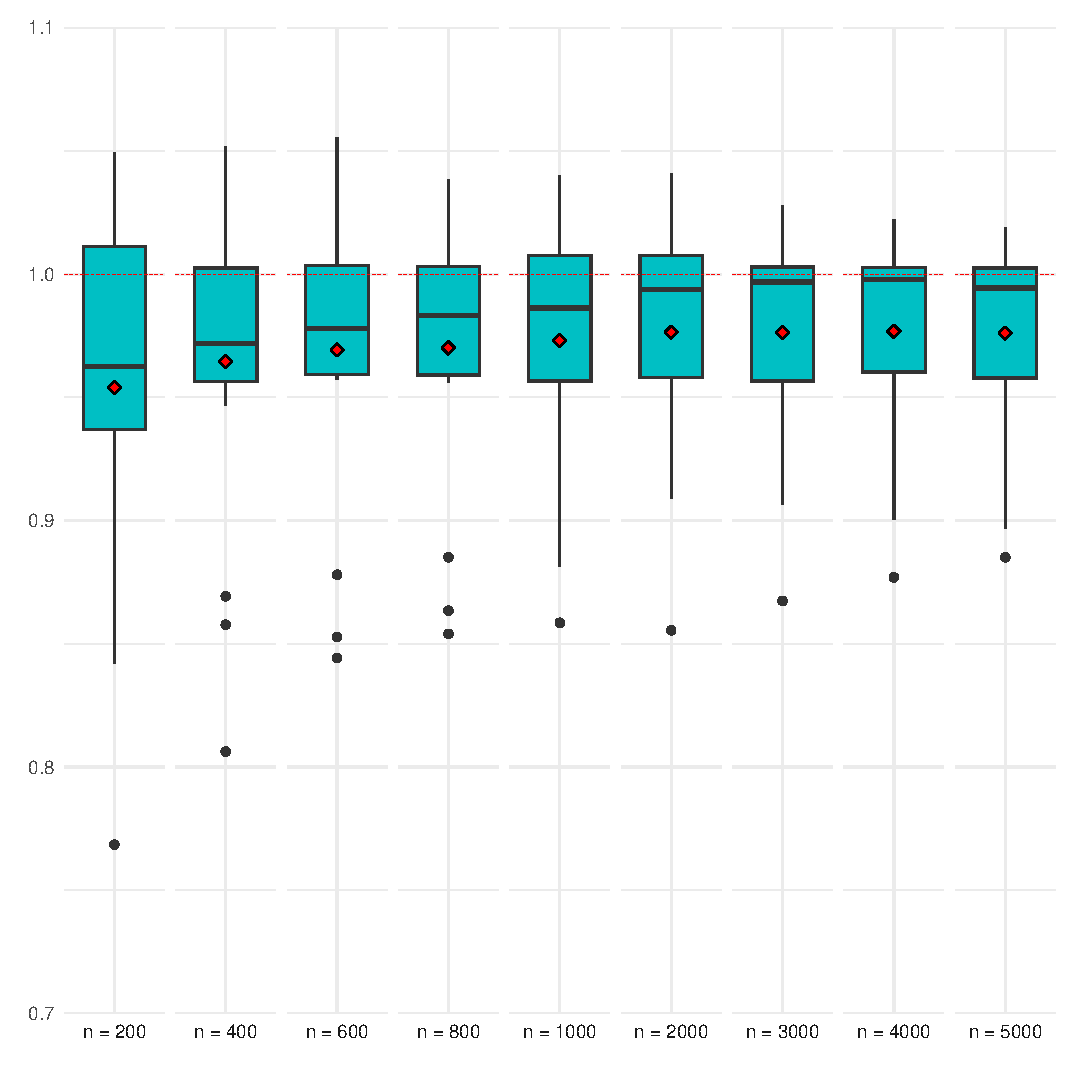
\includegraphics[width=5.5in,height=5in]
{graphs/weighted_rf_rmse_ratios_kappa_2_shrinkage}
\captionof{figure}{Boxplots of  RMSE ratios~\eqref{eq:rmse-rat}. For
  each training-set size $n$, the boxplot is based on the 17~ratios
  corresponding to the datasets listed in Table~\ref{table:datasets}.}
\label{fig:main}
\end{center}

%\tcr{Damian: Do we need to say anything about why the outperformance
 % diminishes as $n$ increases? Like both RF and HRF are `consistent'
 % forecast methods (when data are i.i.d.) and hence the difference
 % between the forecasts vanishes as $n$ increases.}


\subsection{Negative Weights and Shrinkage}
\label{sec:neg-weights}

All previous proposals for weighting the random forest
we are aware of, not only in the context of regression but 
also in the context of classification,
impose the ``no-short-sales constraint'' $\kappa = 1$, that is, $w_j
\ge 0$. As shown in the robustness checks of
Appendix~\ref{app:robust}, allowing for negative weights
typically improves the performance of HRF, and for certain datasets by a pronounced margin, when $\Sigma$ is estimated with nonlinear shrinkage. 
In contrast, this is not the case when the sample covariance
matrix is used to estimate $\Sigma$. To illustrate this finding visually, we consider the following two RMSE ratios:

\begin{equation}\label{eq:rmse-rat-sample-short}
\text{RMSE}_{\kappa=2/\kappa=1}^{\text{sample}} \defeq 
  \frac{
  \sqrt{\frac{1}{B} \sum_{b=1}^B  \text{MSE}_{\text{HRF,b,$\kappa=2$,sample}}}}
  {\sqrt{\frac{1}{B} \sum_{b=1}^B  \text{MSE}_{\text{HRF,b,$\kappa=1$,sample}}}}
\end{equation}
and
\begin{equation}\label{eq:rmse-rat-shrinkage-short}
\text{RMSE}_{\kappa=2/\kappa=1}^{\text{shrinkage}}\defeq 
  \frac{
  \sqrt{\frac{1}{B} \sum_{b=1}^B  \text{MSE}_{\text{HRF,b,$\kappa=2$,shrinkage}}}}
  {\sqrt{\frac{1}{B} \sum_{b=1}^B  \text{MSE}_{\text{HRF,b,$\kappa=1$,shrinkage}}}}~.
\end{equation}

These ratios measure the effect of allowing for negative weights
($\kappa = 2$) relative to imposing non-negative weights ($\kappa =
1$): Ratio~\eqref{eq:rmse-rat-sample-short} does so when $\Sigma$ is
estimated by the sample covariance matrix 
whereas ratio~\eqref{eq:rmse-rat-shrinkage-short}
does so when $\Sigma$ is estimated by nonlinear shrinkage.
Figure \ref{fig:short-selling} shows that allowing for negative weights, in
balance, leads to poorer performance when $\Sigma$ is estimated by the
sample covariance matrix---in contrast to using nonlinear
shrinkage, where it leads to better performance.

This finding might explain to some extent why the
forecast-combination literature, so~far, has generally shied
away from negative weights: It is still the {\em status quo} in
this literature to use the sample covariance
matrix, a practice that should be abandoned.

\textcolor{blue}{%
A portfolio-theoretic perspective helps clarify when negative weights are
most beneficial.
In the minimum-variance portfolio literature it is well known that optimal
weights are all non-negative when the constituent assets are mutually
uncorrelated: independent variance reduction can be achieved without any
short positions.
As pairwise correlations increase, however, negative weights become
necessary to fully exploit diversification---the optimal portfolio ``shorts''
the most redundant assets to cancel shared noise.
The same logic applies to random forest trees.
Trees are explicitly decorrelated via feature subsampling (the
\texttt{mtry} parameter), but this decorrelation is imperfect when the input
features are themselves highly correlated.
In such datasets trees remain substantially correlated, and allowing
$\kappa = 2$ is expected to yield the largest gains over $\kappa = 1$,
because the negative weights cancel the systematic component of prediction
error that the correlated trees share.
Conversely, when features are nearly independent and trees are already
well-decorrelated, the non-negativity constraint ($\kappa = 1$) is
approximately binding without penalty, and the additional flexibility of
$\kappa = 2$ adds little.
This provides an interpretable characterisation of when the hedged random
forest with negative weights is most valuable.
}

In real-life finance applications, a ``no-short-sales constraint'' can be
motivated by legislation (for example, mutual funds are not allowed to
short stocks) or by practical considerations (for example, shorting
certain assets may not be possible or may be prohibitively expensive). On the
other hand, ``short-selling'' individual forecasting methods ${\cal M}_j$ by
assigning them a negative weight does not violate any laws and
does not incur any monetary costs. We therefore hope that this paper will
serve as motivation to allow for negative
weights not only in the random forest but also 
in other forecast-combination settings. Just remember to abandon the
sample covariance matrix in favor of shrinkage estimation of $\Sigma$,
unless the number of forecasting methods is negligible relative to the number of observations in the training set.

\medskip
\begin{center}
\captionsetup{type=figure}
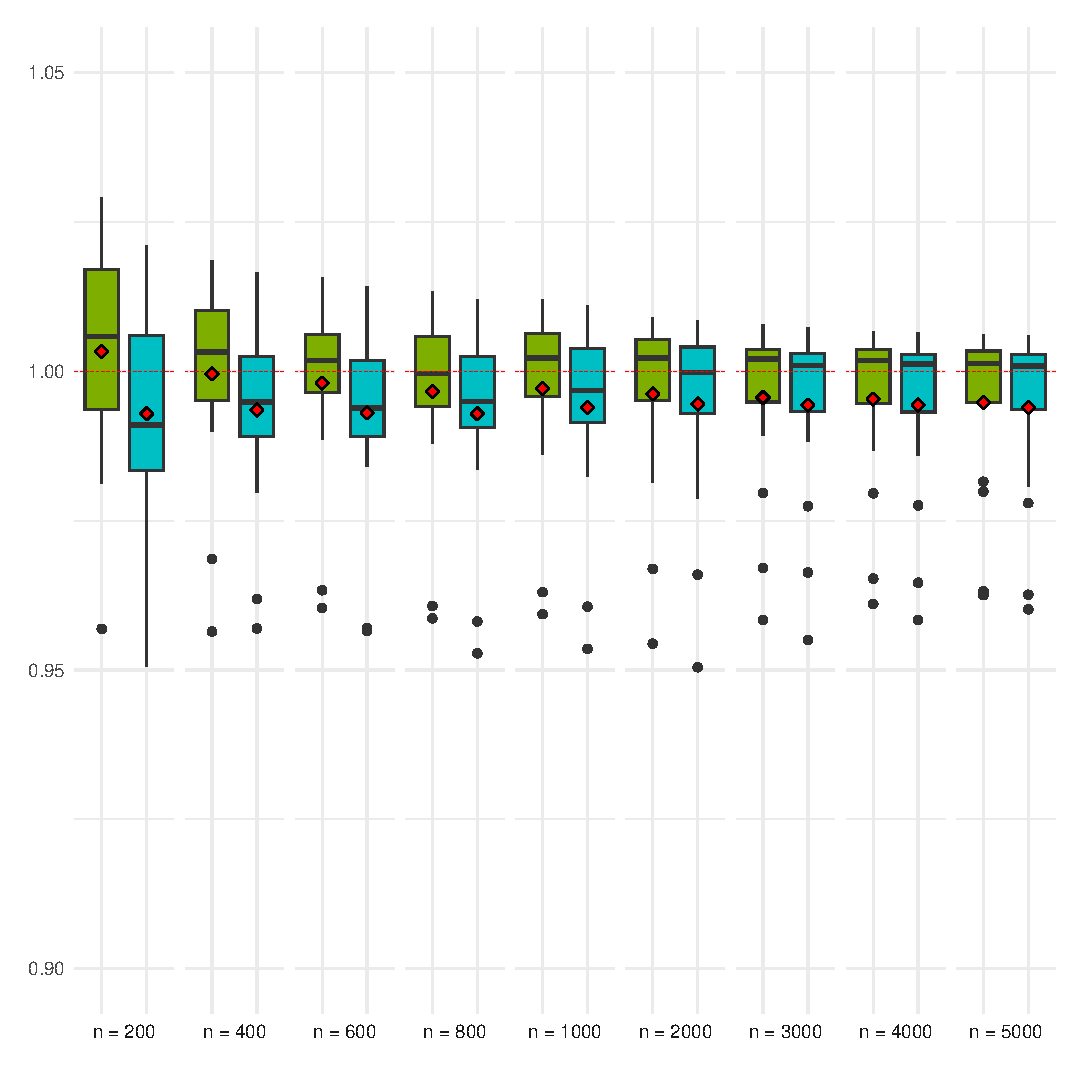
\includegraphics[width=6.01in,height=5in]
{graphs/weighted_rf_rmse_ratios_short_selling}
\captionof{figure}{Boxplots of  RMSE ratios~\eqref{eq:rmse-rat-sample-short} in green and RMSE ratios~\eqref{eq:rmse-rat-shrinkage-short} in blue. For
  each training-set size $n$, the boxplots are based on the 17~ratios
  corresponding to the datasets listed in Table~\ref{table:datasets}.}
\label{fig:short-selling}
\end{center}

\subsection{Related Literature}
There have been previous proposals in the literature for weighting the random forest, so it~is of~interest to compare the~HRF with~them. \textcolor{blue}{We also compare the HRF against general (not random-forest-specific) forecast-combination benchmarks and against a variant of the HRF's own optimization problem.}

\subsubsection{Comparison One}
\label{sec:comp1}
\textcolor{blue}{In this comparison, we consider five alternative weighting or combination
schemes for the random forest.} We first compare the HRF with two
proposals originally intended for the task of classification but
easily adaptable for the task of regression, namely the
weighted random forest (WRF) of \cite{winham:2013} and the
C\'esaro random forest (CRF) of \cite{pham:2020}.
As will be seen below, the weights~$\hat w_j$ in
both proposals are always non-negative; actually, they are always
strictly positive.

For the weighted random forest of \cite{winham:2013}, one first
computes, for $j = 1, \ldots p$,
the tree-accuracy measure
\begin{align}
t\mbox{PE}_j \label{eq:win0} \defeq \frac{1}{|\text{OOB}_j|}
\sum_{i \in \text{OOB}_j} \bigl |y_i - \M_j(x_i)\bigr |~,
\end{align}
where OOB$_j \subset \{1, \ldots, n\}$ denotes the out-of-bag set
corresponding to tree $\M_j$, that~is, the~subset of the
training set not used in the training of the tree.
Next, one computes
relative weights according to one of the three following formulas:
\begin{align}
\hat w_{j, \text{rel}} & \defeq 1 - t\mbox{PE}_j \label{eq:win1} \\
  \hat w_{j, \text{rel}} & \defeq \exp \left (\frac{1}{t\mbox{PE}_j} \right )
              \label{eq:win2}  \\
\hat w_{j, \text{rel}} & \defeq \left (\frac{1}{t\mbox{PE}_j} \right )^\lambda
            \quad \mbox{for some } \lambda > 0 \label{eq:win3}            
\end{align}
Finally, the weights $\{\hat w_j\}$ are forced to sum up to one by setting
$$
\hat w_j \defeq \frac{\hat w_{j, \text{rel}}}{\sum_{l=1}^p \hat w_{l, \text{rel}}}~.
$$
Following the advice of \cite{winham:2013}, we tried as the
leading candidates version~\eqref{eq:win2} and 
version~\eqref{eq:win3} with $\lambda \defeq 5$, of which the former performed
somewhat better and is therefore used below.
We can construct as an analog to \eqref{eq:rmse-rat} the ratio

\begin{equation}\label{eq:rmse-rat-win}
\text{RMSE}_{\text{HRF}/\text{WRF}} \defeq 
  \frac{
  \sqrt{\frac{1}{B} \sum_{b=1}^B  \text{MSE}_{\text{HRF,b}}}}
  {\sqrt{\frac{1}{B} \sum_{b=1}^B  \text{MSE}_{\text{WRF,b}}}}~.
\end{equation}

For the Césaro random forest of \citet{pham:2020}, one uses
the tree-accuracy measures $t\mbox{PE}_j$ defined in \eqref{eq:win0}
to construct the weights, but in a different scheme:
One sorts the
measures $\{t\mbox{PE}_1, \ldots, t\mbox{PE}_p\}$ from smallest to largest
and defines $r_j$ as the order of $t\mbox{PE}_j$ in the sorted
sequence. Hence, if
$
t\mbox{PE}_{(1)} \le  t\mbox{PE}_{(2)} \le \cdots \le t\mbox{PE}_{(p)}
$, we have $t\mbox{PE}_j =  t\mbox{PE}_{(r_j)}$.
Then the relative Césaro weights are defined as
\begin{align}
\hat w_{j, \text{rel}} & \defeq {\sum_{l=r_j}^p }\frac{1}{l} \label{eq:cesaro1}~.           
\end{align}
Finally, the weights $\{\hat w_j\}$ are forced to sum up again to one 
by setting
$$
\hat w_j \defeq \frac{\hat w_{j, \text{rel}}}{\sum_{l=1}^p \hat w_{l, \text{rel}}}~.
$$
We can construct as an analog to \eqref{eq:rmse-rat} the ratio
\begin{equation}\label{eq:rmse-rat-cesaro}
\text{RMSE}_{\text{HRF}/\text{CRF}} \defeq 
  \frac{
  \sqrt{\frac{1}{B} \sum_{b=1}^B  \text{MSE}_{\text{HRF,b}}}}
  {\sqrt{\frac{1}{B} \sum_{b=1}^B  \text{MSE}_{\text{CRF,b}}}}~.
\end{equation}

As an analog to Figure~\ref{fig:main}, we now obtain
Figure~\ref{fig:win} which demonstrates that HRF clearly outperforms~WRF, on
balance. The comparison of HRF with CRF is somewhat more subtle:
Although the two methods exhibit comparable performance in terms of
the median RMSE ratio, HRF consistently outperforms CRF in terms of
the mean RMSE ratio for all training-set sizes~$n$.
Hence, taking everything into account, HRF also outperforms CRF, on balance.\footnote{Appendix \ref{sec:results-in-table-format} presents the RMSE results for all datasets and all methods considered (RF, HRF, WRF, CRF, Ridge, and HRF-MinVar).}

\textcolor{blue}{%
We further benchmark HRF against two combination schemes that are not
specific to random forests. \emph{Ridge} estimates the weights $w$
by ridge-penalized least squares of the training-set labels on the
in-sample tree predictions, subject to $w'\bone = 1$,
with the ridge penalty chosen by AIC. \emph{HRF-MinVar} solves the same optimization
problem~\eqref{eq:mf1}--\eqref{eq:mf3} underlying HRF but with the mean
vector $\hat \mu$ set to zero in the objective, that is, a
pure variance-minimization problem; the (scalar) in-sample bias
$w' \hat \mu$ is then added back to the
resulting forecast. Comparing HRF-MinVar with HRF thus isolates the
incremental contribution of explicitly modeling the bias term in the
mean-variance objective~\eqref{eq:mf1}.
}

\medskip
\begin{center}
\captionsetup{type=figure}
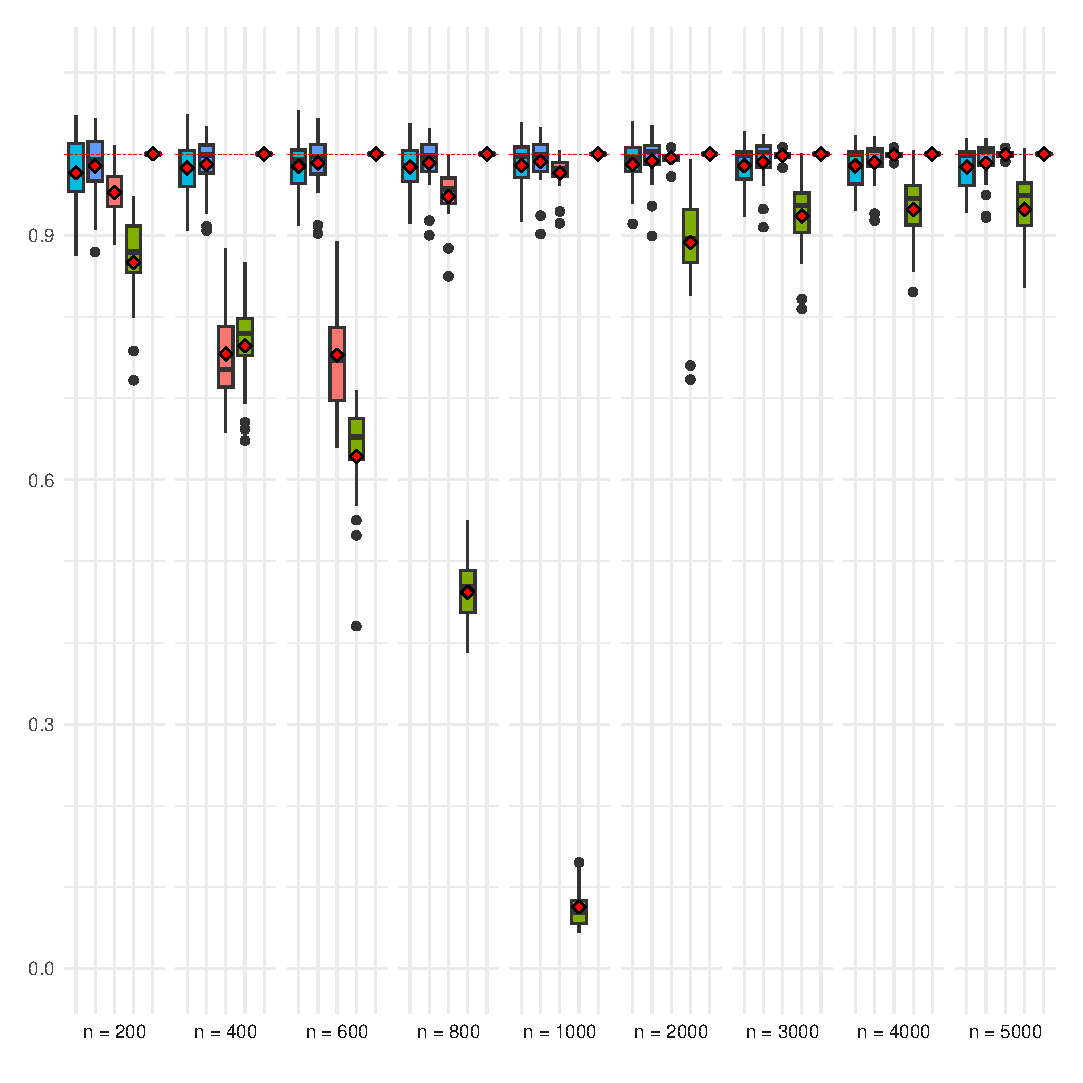
\includegraphics[width=6.01in,height=5in]
{graphs/weighted_rf_rmse_ratios_benchmarks}
\captionof{figure}{Boxplots of  RMSE ratios~\eqref{eq:rmse-rat-win} in light blue and RMSE ratios~\eqref{eq:rmse-rat-cesaro} in dark blue\textcolor{blue}{, together with the analogous RMSE ratios of HRF relative to Ridge (red) and HRF-MinVar (purple)}. For each training-set size $n$, the boxplots are based on the 17~ratios corresponding to the datasets listed in Table~\ref{table:datasets}.}
\label{fig:win}
\end{center}

\textcolor{blue}{%
HRF-MinVar tracks HRF almost exactly (RMSE ratios between 0.999 and 1.001) at
every training-set size, indicating that the variance term in the
mean-variance objective~\eqref{eq:mf1} accounts for virtually all of the
gains over the equal-weighted RF, while the explicit bias term contributes
little once the weights are constrained as in~\eqref{eq:mf2}--\eqref{eq:mf3}.
Ridge is a reasonably strong benchmark but is still dominated by HRF, on
balance, at every training-set size.
}



\subsubsection{Comparison Two}

Next, we compare the HRF with  the proposal of
\cite{chen:yu:zhang:2024}, which has been designed for the task of regression and builds on the framework of \cite{qiu:xie:zhang:2020}.
The latter paper introduces a method for combining the outputs of multiple machine learning algorithms (aka base learners) using weights derived from Mallows-type criteria. \cite{chen:yu:zhang:2024} extend this idea to random forests by treating individual trees as base learners. They prove that, in a certain setting, their approach is asymptotically optimal 
and hence use the acronym $\mbox{WRF}_{\text{opt}}$ which stands 
for ``optimal weighted random forest". 
\cite{chen:yu:zhang:2024} propose two implementations: (i) 1step-WRF\(_{\text{opt}}\), a computationally intensive version, and (ii) 2steps-WRF\(_{\text{opt}}\), a computationally more efficient version, which actually performs better in their empirical application. Consequently, we adopt version 2steps-WRF\(_{opt}\) for our comparison and refer to it as ``optimal weighted random forest" (OWRF).  

We originally wanted to include OWRF in the analysis of Section \ref{sec:comp1} but could not obtain results. 2steps-WRF\(_{\text{opt}}\) is based on quadratic optimization which in practice is carried out with a numerical solver. But this solver does not converge reliably, regardless of whether one uses the hyperparameters for training the random forest as detailed in Section~\ref{sec:hrf} or those proposed by \cite{chen:yu:zhang:2024}, which are detailed below.
The problem remains if one uses 1step-WRF\(_{\text{opt}}\)
instead of 2steps-WRF\(_{\text{opt}}\).

To enable a comparison, we thus use the datasets selected by~\cite{chen:yu:zhang:2024}, which amounts to giving them the ``home field advantage". This is because instead of using a benchmark collection of datasets from the literature, the authors select 12~datasets themselves (without providing the corresponding rationale). Specifically, \cite{chen:yu:zhang:2024} select 11~datasets from the UCI Machine Learning Repository plus an additional dataset from \texttt{openml.org}.
To implement OWRF, we use the code that has been made publicly available by the authors\footnote{See
\href{https://github.com/XinyuChen-hey/Optimal-Weighted-Random-Forests}
{\texttt{https://github.com/XinyuChen-hey/Optimal-Weighted-Random-Forests}}.}
and, surprisingly, differs in certain aspects from the description of the underlying algorithm in the paper.
Following the code of \cite{chen:yu:zhang:2024},
each dataset is randomly partitioned into a training set (70\%) and a testing set (30\%).\footnote{This is in contrast to the paper which states that each dataset is randomly partitioned into a training set (50\%), a testing set (30\%), and a validation set (20\%).} 
In order to guard
against spurious results due to the random partitioning of the data, this process is then repeated (independently) $B=1,000$ times\footnote{\cite{chen:yu:zhang:2024} use $D$ instead of $B$ to denote the number of repetitions.} and the performance measures are then averaged across repetitions, as described below.

Importantly, \cite{chen:yu:zhang:2024} do not use the same hyperparameter choices as we (which are detailed  in~Section~\ref{sec:hrf}). To start with, they only use $p=100$ trees instead of $p=500$ trees; this may be because of the computational expense of their implementation 1step-WRF\(_{\text{opt}}\), which is also included in their empirical application. More importantly, each tree is only grown until a minimum of $\sqrt{n}$~observations remain per leaf (with $n$~denoting the number of training observations). This choice is nonstandard and results in much more ``shallow" trees compared to standard conventions in the literature. When conventional choices for the minimum number of observations remaining per leaf are used, the OWRF~algorithm does not even converge reliably on the 12~datasets selected by the authors themselves. To wit, \cite{chen:yu:zhang:2024} use the same value for the hyperparameter \texttt{mtry} as we do, that is, $d/3$ (rounded down to the nearest integer if necessary).
Hence, the key difference is that they use ``shallow" trees whereas we use ``deep" trees.

In the comparison of forecasting methods, as in \cite{chen:yu:zhang:2024}, we include RF as well as WRF and CRF from Section~\ref{sec:comp1}. \textcolor{blue}{That is, we use the same benchmarks as \cite{chen:yu:zhang:2024}, the paper that proposed this collection of datasets, and add our own method, HRF.} For all three methods, we retain the hyperparameter choices introduced in Section~\ref{sec:hrf} for HRF, as this reflects how applied researchers would typically use these methods in practice.
This is in contrast to \cite{chen:yu:zhang:2024} who retain the OWRF hyperparameter also for RF, WRF, and CRF; this means that, essentially, they compare OWRF with methods that rarely would be used in practice.

\cite{chen:yu:zhang:2024} evaluate forecasting performance using the following two measures:
$$
    \text{MSFE} \defeq \frac{1}{B*n_{\text{test}}} \sum_{b=1}^{B} \sum_{i=1}^{n_{test}} (\hat{y}_{b,i}-y_i)^2 \quad \mbox{and} \quad
    \text{MAFE} \defeq \frac{1}{B*n_{\text{test}}} \sum_{b=1}^{B} \sum_{i=1}^{n_{test}} |\hat{y}_{b,i}-y_i|~,
$$ 
where $B$ denotes the number of data-partition repetitions, 
$\hat{y}_{d,i}$ denotes the forecast  of~$y_i$ in the 
$b^{th}$~repetition, and $n_{\text{test}}$ denotes the sample size of the test data.

Table~\ref{tab:owrf-comparison} presents the results: 
Panel~(a) presents the MSFE~results and 
Panel~(b) presents the MAFE~results.
It can be seen that, in terms of either criterion, HRF stands out as the clear winner, providing the lowest value for~11 out of the 12~datasets. 

Notably, the ``optimal" method OWRF is best zero~times and is not only outperformed by HRF (always) but also by WRF and CRF (on balance).
The latter finding is in contrast to the results in \cite{chen:yu:zhang:2024}, the reason being that the authors retain the nonstandard OWRF hyperparameters also for WRF and CRF.

\begin{table}
\centering
\begin{tabular}{l S S S S S}
\multicolumn{6}{c}{Panel (a): MSFE} \\
\midrule

Dataset & RF & HRF  & OWRF & WRF & CRF \\ 
  \hline
BH & 11.66 &\B 10.26 & 12.01 & 11.00 & 11.09 \\ 
  servo & 1.49 &\B 0.60 & 0.77 & 0.70 & 1.05 \\ 
  CCS & 32.47 &\B 25.39 & 39.35 & 29.00 & 29.45 \\ 
  ASN & 13.27 &\B 5.43 & 12.30 & 8.96 & 10.31 \\ 
  CCPP & 11.56 &\B 11.14 & 14.85 & 11.31 & 11.22 \\ 
  CST & 18.74 &\B 12.10 & 15.57 & 13.74 & 15.69 \\ 
  EE & 2.33 &\B 1.88 & 2.60 & 2.09 & 2.21 \\ 
  PT & 0.26 &\B 0.12 & 0.61 & 0.16 & 0.19 \\ 
  QSAR & 1.25 & 1.28 & 1.34 &\B 1.23 & 1.24 \\ 
  SM & 2.46 &\B 0.88 & 2.25 & 1.30 & 1.87 \\ 
  YH & 17.73 &\B 1.14 & 2.54 & 1.68 & 5.53 \\ 
  tecator & 4.19 &\B 2.63 & 3.28 & 2.65 & 3.09 \\ 
\bottomrule
\addlinespace[5mm]
\multicolumn{6}{c}{Panel (b): MAFE} \\
\midrule

 Dataset & RF & HRF  & OWRF & WRF & CRF \\ 
  \hline
BH & 2.25 &\B 2.16 & 2.36 & 2.20 & 2.21 \\ 
  servo & 0.87 &\B 0.45 & 0.54 & 0.49 & 0.71 \\ 
  CCS & 4.21 &\B 3.57 & 4.82 & 3.93 & 3.98 \\ 
  ASN & 2.94 &\B 1.75 & 2.76 & 2.35 & 2.55 \\ 
  CCPP & 2.47 &\B 2.40 & 2.92 & 2.44 & 2.42 \\ 
  CST & 3.26 &\B 2.62 & 3.00 & 2.80 & 3.00 \\ 
  EE & 0.97 &\B 0.83 & 1.05 & 0.90 & 0.94 \\ 
  PT & 0.34 &\B 0.23 & 0.57 & 0.26 & 0.29 \\ 
  QSAR & 0.82 & 0.83 & 0.85 &\B 0.81 & 0.81 \\ 
  SM & 1.20 &\B 0.68 & 1.13 & 0.84 & 1.03 \\ 
  YH & 2.61 &\B 0.54 & 0.97 & 0.70 & 1.47 \\ 
  tecator & 1.45 &\B 1.09 & 1.31 & 1.18 & 1.27 \\ 
\bottomrule
\end{tabular}
\caption{\small Comparison of five forecasting methods (RF, HRF, OWRF, WRF, and CRF) using two performance criteria (MSFE and MAFE) across 12 datasets. Panel~(a) presents MSFE results and Panel~(b) presents MAFE results. In each row, the lowest (and thus best) value is in {\bf bold face}.}
\label{tab:owrf-comparison}
\end{table}


\begin{remark}[Inability to reproduce exact results]
\label{rem:dorks} \rm 
The reader may observe that the OWRF results in Table \ref{tab:owrf-comparison} differ somewhat from the corresponding 2steps-WRF\(_{\text{opt}}\) results in Tables~3 and~4 of \cite{chen:yu:zhang:2024}. All we can say is that we have faithfully executed the authors' publicly available code. Why the results we obtain do not match those reported in the paper is unclear.~\qed
\end{remark}  

\subsection{Additional Application to Finance}
\label{sec:fredmd}

We have previously demonstrated that the hedged random forest, on
balance, provides superior forecasting performance relative to the
standard random forest{\color{blue}, both for cross-sectional (i.i.d.)\ data (Sections~\ref{sec:results}--\ref{sec:comp1}) and, as we show next, for financial time series}. {\color{blue}Most of our} evidence
has been for cross-sectional (or i.i.d.) datasets.
Such datasets are easy to handle in the sense that we can offer ``one-size-fits-all" estimators of the two inputs required for the hedged random forest, the mean vector $\mu$  and the covariance matrix $\Sigma$ of the vector of forecast errors corresponding to the individual trees. These estimators do not require any user inputs and thus applied researchers only have to ``point and shoot".

Things change in the case of time-series data: What are suitable estimators of $\mu$  and~$\Sigma$ depends on the nature and frequency of the data and on the sample size. Therefore, these estimators have to be custom-tailored to the application at hand. This is unfortunate but also ``par for the course" for time-series applications where ``one-size-fits-all" solutions rarely exist. \cite{beck:wolf:hrf-inf} detail how to adapt the hedged random forest to the specific task of forecasting inflation and demonstrate that it consistently outperforms the standard random forest in terms of forecasting accuracy.

{\color{blue}
As an additional, genuinely financial-econometric application, we adapt the same time-series machinery of \cite{beck:wolf:hrf-inf} to forecast a broad panel of interest-rate, credit-spread, exchange-rate, and price series drawn from the FRED-MD database \citep{mccracken:ng:2016}, a monthly panel of 126 U.S.\ macroeconomic and financial time series maintained by the Federal Reserve Bank of St.\ Louis and updated in real time. We consider two of FRED-MD's eight variable groups, \emph{Interest and Exchange Rates} and \emph{Prices}, for a total of 41 target series: 20~price indices (CPI and PPI sub-indices and the PCE price deflator and its components), 9~interest-rate levels (the federal funds rate, Treasury bills, Treasury and corporate-bond yields), 8~credit and term spreads (relative to the federal funds rate), and 4~exchange rates.

As in \cite{beck:wolf:hrf-inf}, the two inputs $\hat\mu$ and $\hat\Sigma$ required by the HRF (see Section~\ref{sec:hrf}) are estimated from the in-sample tree residuals using an exponentially weighted moving average combined with linear shrinkage toward a constant-variance-covariance target, with the EWMA parameter set to $\lambda=0.15$ and the leverage constraint set to $\kappa=2$, exactly as in \cite{beck:wolf:hrf-inf}. We use a rolling estimation window of 360 months and a random forest of $p=500$ trees with \texttt{mtry}~$=d/3$. Features consist of four lags of every FRED-MD series with a complete history over the estimation window, the first four principal components of that panel (re-estimated within each rolling window), and four autoregressive lags of the target itself. Because the FRED-MD series differ in their statistical nature, we tailor the forecasting target to each series following McCracken and Ng's own classification of the required stationarity-inducing transformation \citep{mccracken:ng:2016}: for the price indices and exchange rates we forecast the one-month percent change and convert the forecast back to the level (analogous to the ``path-average'' approach of \cite{beck:wolf:hrf-inf}); for the interest-rate levels we forecast the one-month change in the rate; and for the (already stationary) credit and term spreads we forecast the spread directly. We restrict attention to the one-month-ahead forecast horizon, $h=1$.

The out-of-sample evaluation period runs from May 1990 through April 2026, yielding $N=432$ monthly forecasts for each of the 41 target series. As before, we report the ratio of the root-mean-squared forecast errors of HRF relative to RF,
\begin{equation}\label{eq:rmse-rat-fredmd}
\text{RMSE}_{\text{HRF}/\text{RF}} \defeq
  \frac{\sqrt{\frac{1}{N}\sum_{t=1}^N \hat e_{t,\text{HRF}}^2}}
       {\sqrt{\frac{1}{N}\sum_{t=1}^N \hat e_{t,\text{RF}}^2}}~,
\end{equation}
where $\hat e_{t,\text{HRF}}$ and $\hat e_{t,\text{RF}}$ denote the forecast errors of HRF and RF, respectively, at month~$t$; a ratio below one indicates that HRF outperforms RF.

% latex table generated by src/analysis/fredmd_analysis.R
\begin{table}[ht]
\centering
\begin{tabular}{lrrrr}
\toprule
\textbf{Group} & \textbf{$N$} & \textbf{Mean ratio} & \textbf{Median ratio} & \textbf{Share ratio $<1$} \\
\midrule
Prices & 20 & 0.991 & 0.990 & 85\% \\
Interest rates & 9 & 0.995 & 0.992 & 56\% \\
Credit/term spreads & 8 & 0.938 & 0.939 & 100\% \\
Exchange rates & 4 & 1.000 & 1.001 & 50\% \\
\midrule
All series & 41 & 0.982 & 0.988 & 78\% \\
\bottomrule
\end{tabular}
\caption{RMSE ratios \eqref{eq:rmse-rat-fredmd} of the hedged random forest relative to the standard random forest, by FRED-MD group, horizon $h=1$. \emph{Share ratio $<1$} is the fraction of series within the group for which HRF achieves a lower RMSE than RF. Full per-series results are in Appendix~\ref{sec:results-in-table-format}, Table~\ref{tab:fredmd-detail}.}
\label{table:fredmd-summary}
\end{table}


Table~\ref{table:fredmd-summary} presents the results, aggregated by group; the full breakdown for all 41 series is provided in Appendix~\ref{sec:results-in-table-format}, Table~\ref{tab:fredmd-detail}. Across all 41 series, the mean RMSE ratio is~0.982 and HRF achieves a lower RMSE than RF for 32 of the 41 series (78\%). The gains are strongest and most uniform for the eight credit and term spreads, where HRF wins for every single series, with a mean RMSE ratio of~0.938. The gains are more modest, but still favor HRF, for the 20 price indices (mean ratio~0.991, 85\% of series improved). Results are mixed for the 9 interest-rate levels (mean ratio~0.995, 56\% of series improved): the improvement is concentrated in short-term rates (the federal funds rate, commercial paper, and Treasury bills up to one year), whereas for longer-maturity Treasury and corporate-bond yields RF performs (slightly) better. For the four exchange rates the two methods are essentially tied (mean ratio~1.000), consistent with the well-documented difficulty of beating a random walk in exchange-rate forecasting.

\medskip
\begin{center}
\captionsetup{type=figure}
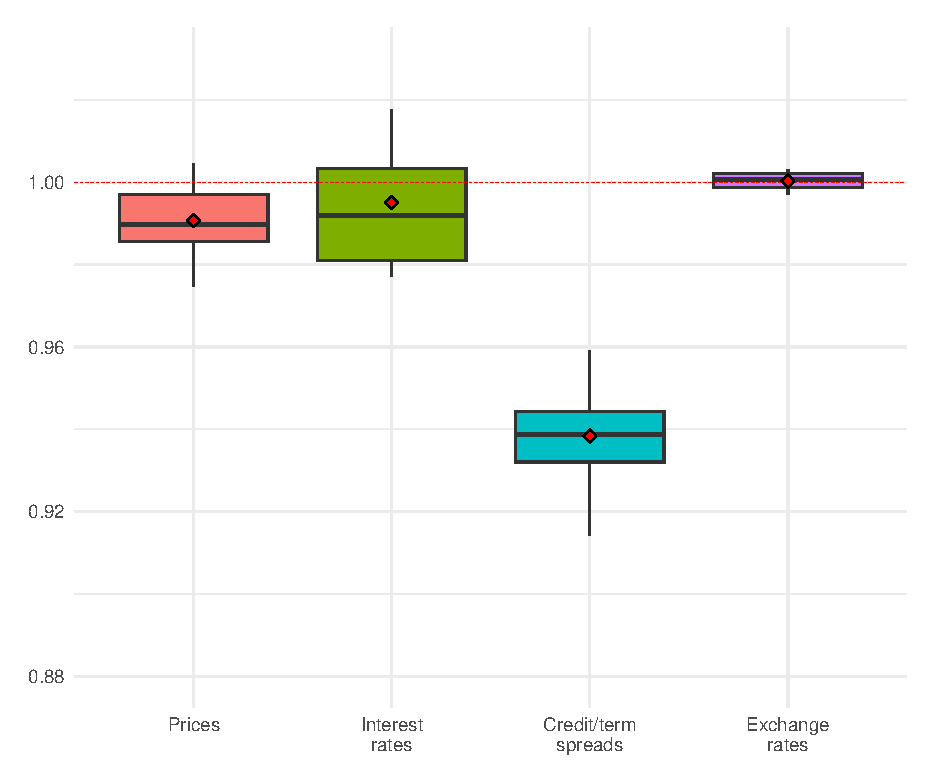
\includegraphics[width=6.01in,height=5in]
{graphs/fredmd_rmse_ratios_boxplot}
\captionof{figure}{Boxplots of RMSE ratios~\eqref{eq:rmse-rat-fredmd} by FRED-MD group. The diamond marks the group mean, and the dashed line marks the parity value of one; values below one indicate that HRF outperforms RF. Each boxplot is based on the RMSE ratios of the series in that group (20 for Prices, 9 for Interest rates, 8 for Credit/term spreads, 4 for Exchange rates), listed individually in Appendix~\ref{sec:results-in-table-format}, Table~\ref{tab:fredmd-detail}.}
\label{fig:fredmd-boxplot}
\end{center}
}

\section{Conclusion}

Machine learning (ML) methods have become an important empirical tool for virtually all empirically oriented researchers in economics and finance.  In particular, the random forest is one of the most popular and widely employed supervised machine learning methods. It is especially suitable for applications in economics and finance, where datasets are generally still ``small to medium sized`` by machine learning standards;
for example, see \citet{grinsztajn:2022} and
\cite{januschowski2022forecasting}.

This paper has focused on the scenario where the random forest is used to forecast a numerical variable, that is, on the task of regression. In its standard form, the random forest is an equal-weighted ensemble of individual trees. We have suggested a weighting scheme where the weights still sum up to one but are no longer equal and may even be negative. Our scheme borrows certain ideas from financial portfolio selection. In particular, we impose an upper bound on the $L_1$~norm of the vector of weights (that is, on the sum of the absolute values of the weights), which ``hedges" the user against weights that are unduly large in absolute value.
As a consequence, we call the proposal the {\em hedged random forest}. It should be noted that our scheme for weighting individual forecasts is of high-level nature and can be applied to any generic forest-combination problem, of which the random forest is essentially a special case.

An extensive empirical analysis has demonstrated that the hedged random forest not only outperforms the standard random forest in terms of forecasting accuracy but also three previous proposals from the machine learning literature for weighted random forests (all of which only employ non-negative weights of the individual trees).

There are (at least) three fruitful avenues for future research. First, study the benefits of the hedged random forest relative to the standard random forest when the latter is not used for forecasting but for other purposes such as the estimation of treatment and causal effects; for example, see \cite{athey:imbens:2016} and \cite{wager:athey:2018}.
Second, study the possibility of hedging the generalized random forest, which can be used to fit any quantity of interest identified as the solution to a set of local moment equations; see \cite{athey:tibshirani:wager:2019}. Third, study the applicability of the hedged random forest for the task of classification, which is related to the task of regression but comes with additional difficulties due to the discontinuous 0-1 loss.

\newpage

\bibliographystyle{apalike}    
% \bibliography{../../wolf}
\bibliography{wolf}

\newpage

\begin{appendix}
\section{Robustness Checks}
  \label{app:robust}

The goal of this appendix is to provide robustness checks regarding
 the nature of the \mbox{estimator $\hat \Sigma$} and the choice of the
gross-exposure constraint $\kappa$.

As an alternative estimator $\hat \Sigma$ to nonlinear shrinkage,
we will consider the
canonical choice, the sample covariance matrix.
 In terms of $\kappa$, we will consider the
choices $\kappa \in \{1, 1.5, 2, 2.5, \infty\}$., the canonical
choice in the forecast-combination literature being $\kappa = 1$.

Figure~\ref{fig:all-kappa-nls} displays the results for all choices of
$\kappa$ when $\hat \Sigma$ is given by nonlinear shrinkage, whereas
Figure~\ref{fig:all-kappa-sample} displays analogous results when
nonlinear shrinkage is replaced by the sample covariance matrix.


\begin{center}
\captionsetup{type=figure}
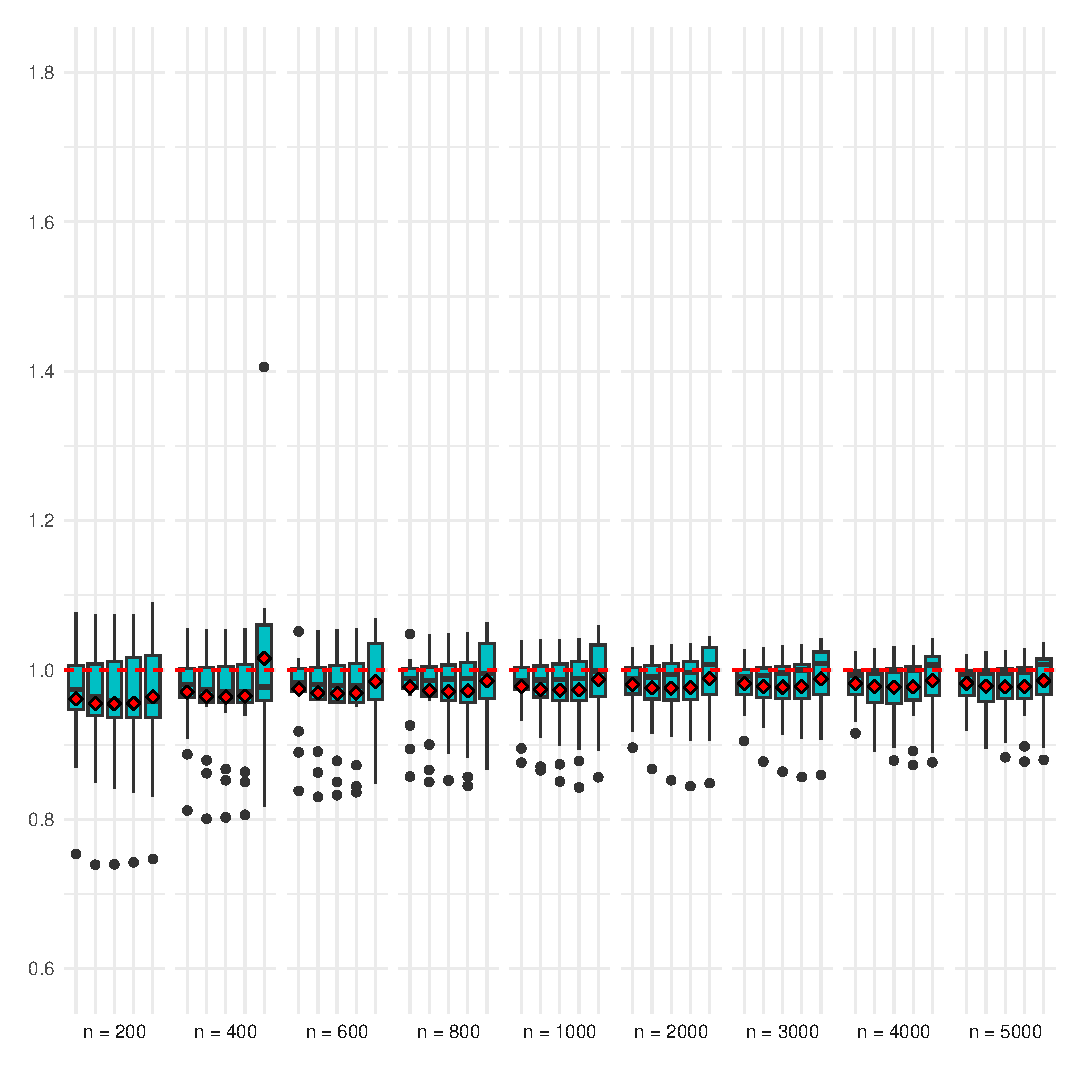
\includegraphics[width=6.01in,height=5in]
{graphs/weighted_rf_rmse_ratios_appendix_shrinkage}
\captionof{figure}{Boxplots of  RMSE ratios~\eqref{eq:rmse-rat}. For
  each training-set size $n$, there are five boxplots corresponding to
  $\kappa \in \{1, 1.5, 2, 2.5, \infty\}$ where
  each boxplot is based on the 17~ratios
  corresponding to the datasets listed in Table~\ref{table:datasets}.
  The estimator $\hat \Sigma$ is given by nonlinear shrinkage.}
\label{fig:all-kappa-nls}
\end{center}

\begin{center}
\captionsetup{type=figure}
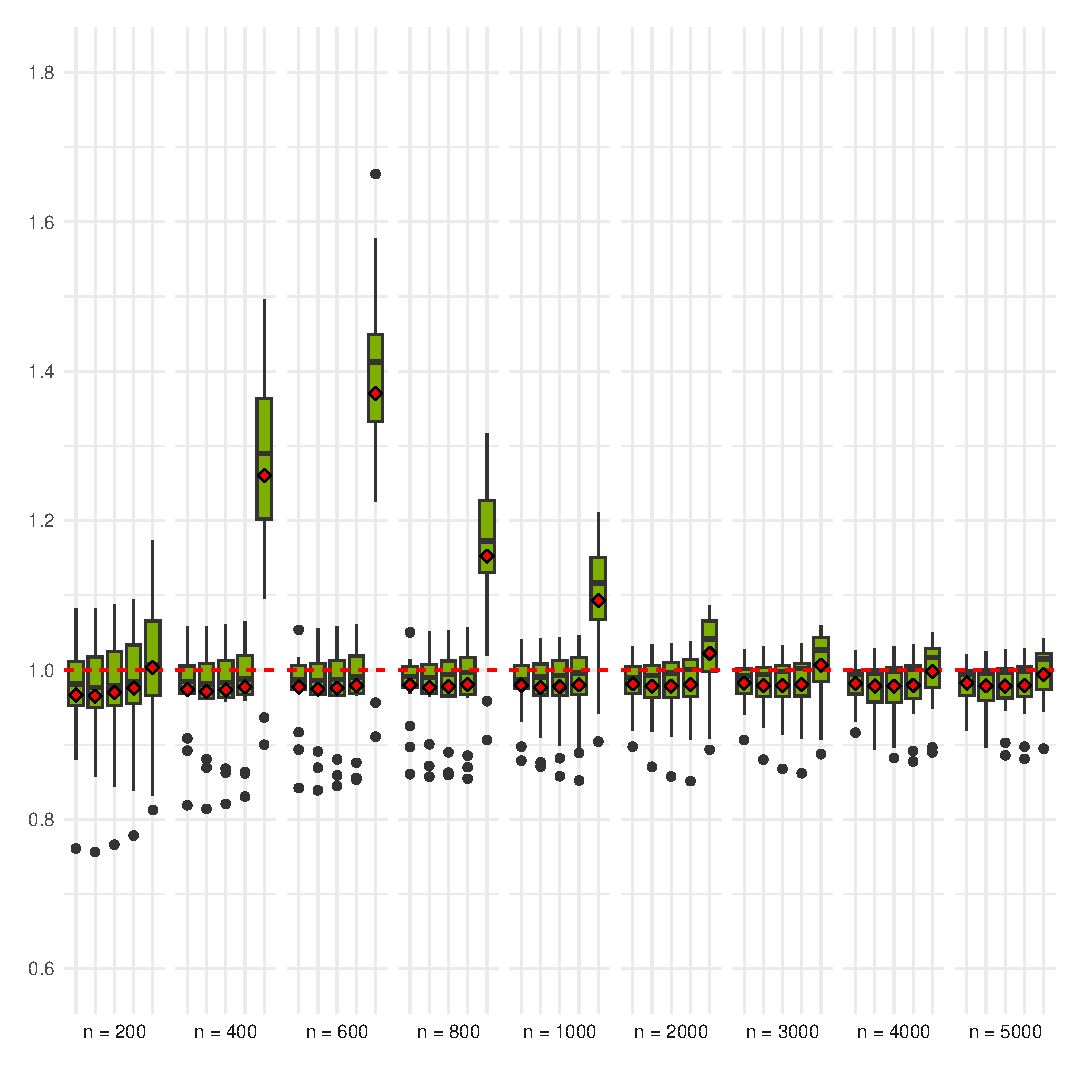
\includegraphics[width=6.01in,height=5in]
{graphs/weighted_rf_rmse_ratios_appendix_sample}
\captionof{figure}{Boxplots of  RMSE ratios~\eqref{eq:rmse-rat}. For
  each training-set size $n$, there are five boxplots corresponding to
  $\kappa \in \{1, 1.5, 2, 2.5, \infty\}$ where
  each boxplot is based on the 17~ratios
  corresponding to the datasets listed in Table~\ref{table:datasets}.
  The estimator $\hat \Sigma$ is given by the sample covariance matrix.}
\label{fig:all-kappa-sample}
\end{center}

When $\hat \Sigma$ is given by nonlinear shrinkage, the choice $\kappa
\in \{1.5, 2, 2.5\}$ matters very little, and all three choices
perform better than
the canonical choice $\kappa = 1$. Not imposing a
gross-exposure constraint (that~is, the choice $\kappa = \infty)$
performs worst overall, although it still outperforms RF, on balance.

When $\hat \Sigma$ is given by the sample covariance matrix instead,
the choice of $\kappa$ matters more. In particular, not imposing a
gross-exposure constraint (that is, the choice $\kappa = \infty)$
can lead to grave underperformance of the HRF when the training-set
size, $n$, is close~to the~number of trees, $p$. Overall, the
choice $\kappa = 1$ seems to perform best.

Finally, we look at the combined benefit of our version of HRF
compared to the {\em status~quo} in the 
forecast-combination literature: This means that (i) we use nonlinear
shrinkage for $\hat \Sigma$ instead of the sample covariance matrix
and (ii) we use $\kappa = 2$ instead of $\kappa = 1$.
Calling the two versions HRFour and HRFcan (for ``our'' and
``canonical''),
we can construct as an analog to \eqref{eq:rmse-rat} the ratio

\begin{equation}\label{eq:rmse-rat-can}
\text{RMSE}_{\text{HRFour}/\text{HRFcan}} \defeq 
  \frac{
  \sqrt{\frac{1}{B} \sum_{b=1}^B  \text{MSE}_{\text{HRFour,b}}}}
  {\sqrt{\frac{1}{B} \sum_{b=1}^B  \text{MSE}_{\text{HRFcan,b}}}}~.
\end{equation}

As an analog to Figure~\ref{fig:main} we then obtain
Figure~\ref{fig:can},
\medskip
\begin{center}
\captionsetup{type=figure}
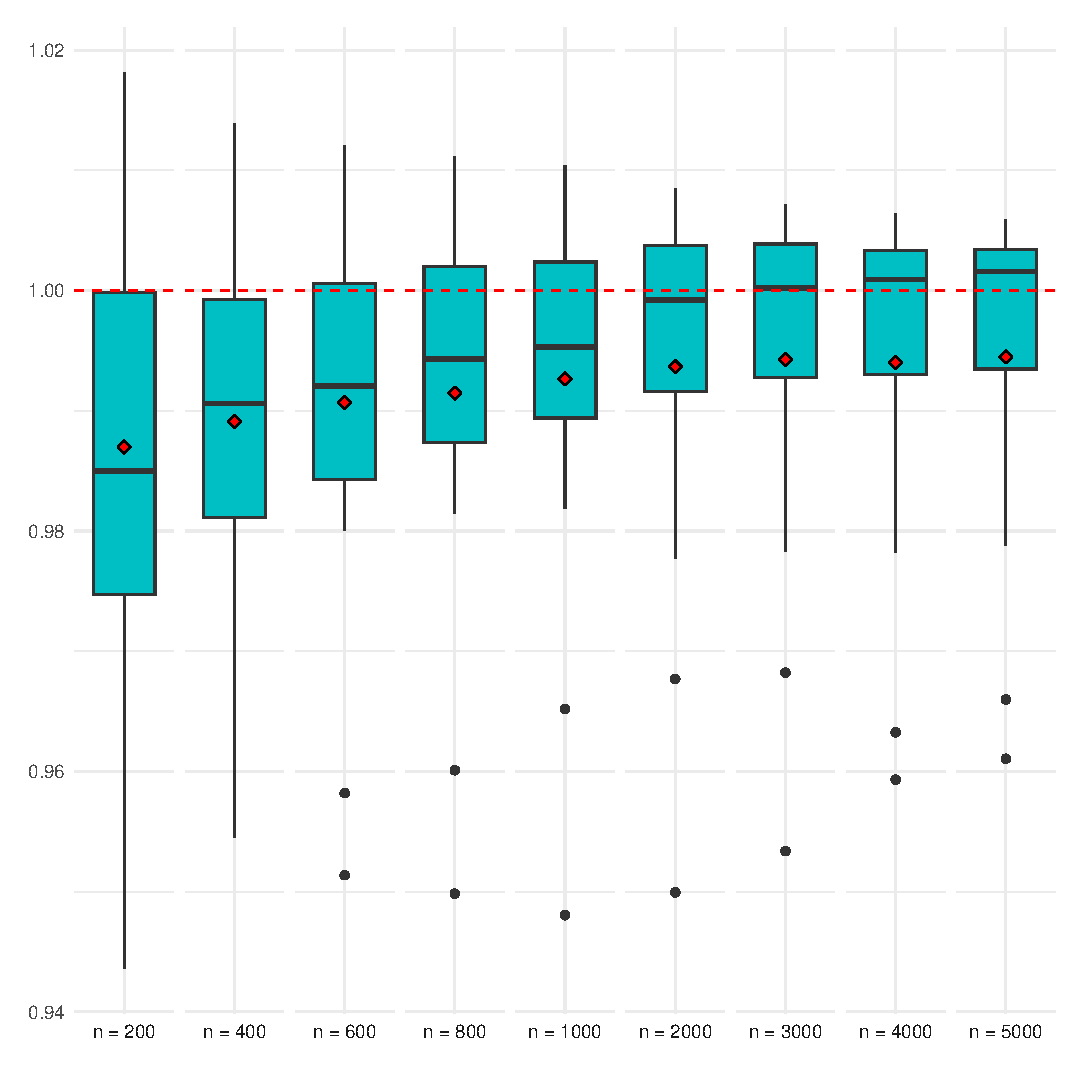
\includegraphics[width=6.01in,height=5in]
{graphs/weighted_rf_rmse_ratios_shrinkage_2_sample_1.eps}
\captionof{figure}{Boxplots of  RMSE ratios~\eqref{eq:rmse-rat-can}. For
  each training-set size $n$, the boxplot is based on the 17~ratios
  corresponding to the datasets listed in Table~\ref{table:datasets}.}
\label{fig:can}
\end{center}

One can see that in~terms of the median RMSE ratio,
our version outperforms the
canonical version for $n \le 2000$, after which the competition becomes a tie,
whereas in~terms of the mean RMSE ratio, 
our version outperforms the canonical version for all $n$.

\newpage

\section{Detailed Results in Table Format}
\label{sec:results-in-table-format}
This appendix presents the RMSE results for all datasets, training-set sizes, and forecasting methods discussed in Sections~\ref{sec:results} and \ref{sec:comp1}\textcolor{blue}{, including the Ridge and HRF-MinVar benchmarks of Section~\ref{sec:comp1}}.
\label{sec:results-table-format}
% latex table generated in R 4.2.2 by xtable 1.8-8 package
% Mon Jul  6 13:17:42 2026
\begin{table}[ht]
\centering
\begingroup\scriptsize
\begin{tabular}{lrrrrrr}
  \hline
\textbf{ Name } & \textbf{ RF } & \textbf{ HRF } & \textbf{ WRF } & \textbf{ CRF } & \textbf{ Ridge } & \textbf{ HRF-MinVar } \\ 
  \hline
Ailerons & 0.23 & 0.22 & 0.23 & 0.22 & 0.23 & \textbf{0.22} \\ 
  Bike\_Sharing\_Demand & 126.06 & 125.55 & 125.41 & \textbf{123.91} & 135.05 & 125.51 \\ 
  brazilian\_houses & 0.17 & 0.14 & 0.16 & 0.16 & \textbf{0.14} & 0.14 \\ 
  cpu\_act & 4.21 & 3.65 & 3.75 & 3.66 & 4.06 & \textbf{3.65} \\ 
  diamonds & \textbf{0.26} & 0.28 & 0.26 & 0.26 & 0.31 & 0.28 \\ 
  elevators & 4.78 & 4.72 & 4.77 & 4.75 & 4.90 & \textbf{4.72} \\ 
  house\_16H & \textbf{0.70} & 0.72 & 0.70 & 0.70 & 0.74 & 0.72 \\ 
  house\_sales & 0.26 & 0.25 & 0.26 & 0.26 & 0.27 & \textbf{0.25} \\ 
  houses & 0.37 & 0.36 & 0.37 & 0.36 & 0.37 & \textbf{0.36} \\ 
  isolet & 5.68 & \textbf{5.32} & 5.64 & 5.50 & 5.47 & 5.32 \\ 
  medical\_charges & 0.16 & \textbf{0.12} & 0.13 & 0.13 & 0.13 & 0.12 \\ 
  MiamiHousing2016 & 0.28 & 0.26 & 0.27 & 0.27 & 0.27 & \textbf{0.26} \\ 
  nyc-taxi-green-dec-2016 & 0.50 & 0.52 & 0.50 & \textbf{0.50} & 0.56 & 0.52 \\ 
  pol & 16.60 & 13.99 & 15.97 & 15.20 & 14.17 & \textbf{13.98} \\ 
  sulfur & 0.04 & \textbf{0.03} & 0.04 & 0.03 & 0.04 & 0.03 \\ 
  superconduct & 17.37 & 17.57 & 17.34 & \textbf{17.31} & 18.18 & 17.55 \\ 
  wine\_quality & 0.74 & 0.77 & \textbf{0.74} & 0.75 & 0.81 & 0.77 \\ 
   \hline
\end{tabular}
\endgroup
\caption{Results for all data sets with n = 200. Values for the Ailerons and elevators data sets are scaled by a factor of 1,000 for better readability.} 
\end{table}

% latex table generated in R 4.2.2 by xtable 1.8-8 package
% Mon Jul  6 13:17:42 2026
\begin{table}[ht]
\centering
\begingroup\scriptsize
\begin{tabular}{lrrrrrr}
  \hline
\textbf{ Name } & \textbf{ RF } & \textbf{ HRF } & \textbf{ WRF } & \textbf{ CRF } & \textbf{ Ridge } & \textbf{ HRF-MinVar } \\ 
  \hline
Ailerons & 0.21 & 0.20 & 0.21 & 0.21 & 0.28 & \textbf{0.20} \\ 
  Bike\_Sharing\_Demand & 119.70 & 118.88 & 119.19 & \textbf{117.58} & 169.82 & 118.89 \\ 
  brazilian\_houses & 0.15 & 0.13 & 0.14 & 0.14 & 0.15 & \textbf{0.13} \\ 
  cpu\_act & 3.17 & 3.07 & 3.09 & 3.07 & 4.67 & \textbf{3.07} \\ 
  diamonds & \textbf{0.26} & 0.27 & 0.26 & 0.26 & 0.40 & 0.27 \\ 
  elevators & 4.42 & 4.30 & 4.41 & 4.38 & 5.66 & \textbf{4.30} \\ 
  house\_16H & \textbf{0.68} & 0.71 & 0.68 & 0.69 & 0.85 & 0.71 \\ 
  house\_sales & 0.24 & 0.24 & 0.24 & 0.24 & 0.32 & \textbf{0.24} \\ 
  houses & 0.34 & 0.33 & 0.34 & 0.33 & 0.46 & \textbf{0.33} \\ 
  isolet & 4.83 & \textbf{4.57} & 4.79 & 4.68 & 5.80 & 4.57 \\ 
  medical\_charges & 0.13 & \textbf{0.11} & 0.11 & 0.12 & 0.16 & 0.11 \\ 
  MiamiHousing2016 & 0.24 & 0.23 & 0.24 & 0.24 & 0.31 & \textbf{0.23} \\ 
  nyc-taxi-green-dec-2016 & 0.49 & 0.51 & 0.49 & \textbf{0.49} & 0.69 & 0.51 \\ 
  pol & 13.20 & 11.32 & 12.24 & 12.42 & 13.35 & \textbf{11.31} \\ 
  sulfur & 0.03 & 0.03 & 0.03 & \textbf{0.03} & 0.04 & 0.03 \\ 
  superconduct & 15.66 & 15.70 & 15.63 & \textbf{15.59} & 17.97 & 15.70 \\ 
  wine\_quality & 0.72 & 0.74 & \textbf{0.72} & 0.72 & 1.02 & 0.74 \\ 
   \hline
\end{tabular}
\endgroup
\caption{Results for all data sets with n = 400. Values for the Ailerons and elevators data sets are scaled by a factor of 1,000 for better readability.} 
\end{table}

% latex table generated in R 4.2.2 by xtable 1.8-8 package
% Fri Jul  3 15:26:13 2026
\begin{table}[ht]
\centering
\begingroup\scriptsize
\begin{tabular}{lrrrrrrr}
  \hline
\textbf{ Name } & \textbf{ RF } & \textbf{ HRF } & \textbf{ WRF } & \textbf{ CRF } & \textbf{ Ridge } & \textbf{ 2-Step Ridge } & \textbf{ HRF-MinVar } \\ 
  \hline
Ailerons & 0.20 & 0.20 & 0.20 & 0.20 & 0.26 & 0.30 & \textbf{0.20} \\ 
  Bike\_Sharing\_Demand & 116.30 & 115.64 & 115.88 & \textbf{114.33} & 180.73 & 177.29 & 115.61 \\ 
  brazilian\_houses & 0.14 & 0.12 & 0.14 & 0.14 & 0.14 & 0.18 & \textbf{0.12} \\ 
  cpu\_act & 2.96 & 2.92 & 2.93 & 2.92 & 4.33 & 5.30 & \textbf{2.92} \\ 
  diamonds & \textbf{0.26} & 0.26 & 0.26 & 0.26 & 0.37 & 0.50 & 0.26 \\ 
  elevators & 4.24 & \textbf{4.08} & 4.23 & 4.19 & 5.33 & 6.51 & 4.08 \\ 
  house\_16H & \textbf{0.66} & 0.70 & 0.66 & 0.67 & 0.83 & 0.99 & 0.70 \\ 
  house\_sales & 0.23 & 0.23 & 0.23 & \textbf{0.23} & 0.30 & 0.35 & 0.23 \\ 
  houses & 0.33 & 0.31 & 0.33 & 0.32 & 0.42 & 0.47 & \textbf{0.31} \\ 
  isolet & 4.42 & 4.24 & 4.39 & 4.31 & 5.36 & 6.28 & \textbf{4.24} \\ 
  medical\_charges & 0.12 & \textbf{0.10} & 0.11 & 0.11 & 0.15 & 0.18 & 0.10 \\ 
  MiamiHousing2016 & 0.23 & 0.22 & 0.23 & 0.23 & 0.30 & 0.33 & \textbf{0.22} \\ 
  nyc-taxi-green-dec-2016 & 0.49 & 0.50 & 0.49 & \textbf{0.48} & 0.67 & 0.80 & 0.50 \\ 
  pol & 11.81 & 10.07 & 10.91 & 11.16 & 14.59 & 14.34 & \textbf{10.07} \\ 
  sulfur & 0.03 & 0.03 & 0.03 & \textbf{0.03} & 0.04 & 0.05 & 0.03 \\ 
  superconduct & 14.79 & 14.85 & 14.77 & \textbf{14.73} & 17.27 & 35.31 & 14.84 \\ 
  wine\_quality & 0.71 & 0.72 & \textbf{0.71} & 0.71 & 1.03 & 1.15 & 0.72 \\ 
   \hline
\end{tabular}
\endgroup
\caption{Results for all data sets with n = 600. Values for the Ailerons and elevators data sets are scaled by a factor of 1,000 for better readability.} 
\end{table}

% latex table generated in R 4.2.2 by xtable 1.8-8 package
% Fri Jul  3 15:26:13 2026
\begin{table}[ht]
\centering
\begingroup\scriptsize
\begin{tabular}{lrrrrrrr}
  \hline
\textbf{ Name } & \textbf{ RF } & \textbf{ HRF } & \textbf{ WRF } & \textbf{ CRF } & \textbf{ Ridge } & \textbf{ 2-Step Ridge } & \textbf{ HRF-MinVar } \\ 
  \hline
Ailerons & 0.20 & 0.19 & 0.19 & 0.19 & 0.20 & 0.41 & \textbf{0.19} \\ 
  Bike\_Sharing\_Demand & 114.41 & 113.88 & 114.06 & \textbf{112.62} & 134.02 & 243.17 & 113.84 \\ 
  brazilian\_houses & 0.13 & 0.12 & 0.13 & 0.13 & 0.12 & 0.21 & \textbf{0.12} \\ 
  cpu\_act & 2.88 & 2.85 & 2.86 & 2.86 & 3.07 & 7.20 & \textbf{2.85} \\ 
  diamonds & \textbf{0.25} & 0.26 & 0.25 & 0.25 & 0.26 & 0.65 & 0.26 \\ 
  elevators & 4.11 & \textbf{3.95} & 4.11 & 4.06 & 4.12 & 9.03 & 3.95 \\ 
  house\_16H & \textbf{0.65} & 0.68 & 0.65 & 0.66 & 0.69 & 1.33 & 0.68 \\ 
  house\_sales & 0.23 & 0.22 & 0.23 & \textbf{0.22} & 0.23 & 0.49 & 0.22 \\ 
  houses & 0.32 & 0.30 & 0.32 & 0.31 & 0.31 & 0.64 & \textbf{0.30} \\ 
  isolet & 4.17 & \textbf{4.03} & 4.15 & 4.08 & 4.18 & 8.16 & 4.03 \\ 
  medical\_charges & 0.12 & \textbf{0.10} & 0.10 & 0.11 & 0.11 & 0.25 & 0.10 \\ 
  MiamiHousing2016 & 0.22 & 0.21 & 0.22 & 0.22 & 0.23 & 0.43 & \textbf{0.21} \\ 
  nyc-taxi-green-dec-2016 & 0.48 & 0.49 & 0.48 & \textbf{0.48} & 0.52 & 1.10 & 0.49 \\ 
  pol & 10.97 & \textbf{9.37} & 10.23 & 10.40 & 10.60 & 17.69 & 9.37 \\ 
  sulfur & 0.03 & 0.03 & 0.03 & \textbf{0.03} & 0.03 & 0.06 & 0.03 \\ 
  superconduct & 14.25 & 14.29 & 14.23 & \textbf{14.19} & 15.30 & 36.84 & 14.29 \\ 
  wine\_quality & 0.70 & 0.71 & \textbf{0.70} & 0.70 & 0.74 & 1.55 & 0.71 \\ 
   \hline
\end{tabular}
\endgroup
\caption{Results for all data sets with n = 800. Values for the Ailerons and elevators data sets are scaled by a factor of 1,000 for better readability.} 
\end{table}

% latex table generated in R 4.2.2 by xtable 1.8-8 package
% Mon Jul  6 13:17:42 2026
\begin{table}[ht]
\centering
\begingroup\scriptsize
\begin{tabular}{lrrrrrr}
  \hline
\textbf{ Name } & \textbf{ RF } & \textbf{ HRF } & \textbf{ WRF } & \textbf{ CRF } & \textbf{ Ridge } & \textbf{ HRF-MinVar } \\ 
  \hline
Ailerons & 0.19 & \textbf{0.19} & 0.19 & 0.19 & 0.19 & 0.19 \\ 
  Bike\_Sharing\_Demand & 112.91 & 112.60 & 112.60 & \textbf{111.26} & 123.07 & 112.55 \\ 
  brazilian\_houses & 0.13 & 0.11 & 0.12 & 0.12 & \textbf{0.11} & 0.11 \\ 
  cpu\_act & 2.82 & \textbf{2.80} & 2.81 & 2.80 & 2.88 & 2.80 \\ 
  diamonds & \textbf{0.25} & 0.26 & 0.25 & 0.25 & 0.26 & 0.26 \\ 
  elevators & 4.00 & \textbf{3.82} & 4.00 & 3.95 & 3.87 & 3.83 \\ 
  house\_16H & \textbf{0.65} & 0.67 & 0.65 & 0.65 & 0.68 & 0.67 \\ 
  house\_sales & 0.22 & 0.22 & 0.22 & \textbf{0.22} & 0.22 & 0.22 \\ 
  houses & 0.31 & 0.30 & 0.31 & 0.30 & 0.30 & \textbf{0.30} \\ 
  isolet & 4.01 & \textbf{3.88} & 3.99 & 3.92 & 3.95 & 3.88 \\ 
  medical\_charges & 0.11 & \textbf{0.10} & 0.10 & 0.10 & 0.10 & 0.10 \\ 
  MiamiHousing2016 & 0.21 & 0.20 & 0.21 & 0.21 & 0.21 & \textbf{0.20} \\ 
  nyc-taxi-green-dec-2016 & 0.48 & 0.49 & 0.48 & \textbf{0.48} & 0.50 & 0.49 \\ 
  pol & 10.21 & 8.76 & 9.56 & 9.72 & 9.43 & \textbf{8.76} \\ 
  sulfur & 0.03 & 0.03 & 0.03 & \textbf{0.03} & 0.03 & 0.03 \\ 
  superconduct & 13.81 & 13.92 & 13.80 & \textbf{13.77} & 14.47 & 13.92 \\ 
  wine\_quality & 0.69 & 0.70 & \textbf{0.69} & 0.69 & 0.71 & 0.70 \\ 
   \hline
\end{tabular}
\endgroup
\caption{Results for all data sets with n = 1000. Values for the Ailerons and elevators data sets are scaled by a factor of 1,000 for better readability.} 
\end{table}

% latex table generated in R 4.2.2 by xtable 1.8-8 package
% Mon Jul  6 13:17:42 2026
\begin{table}[ht]
\centering
\begingroup\scriptsize
\begin{tabular}{lrrrrrr}
  \hline
\textbf{ Name } & \textbf{ RF } & \textbf{ HRF } & \textbf{ WRF } & \textbf{ CRF } & \textbf{ Ridge } & \textbf{ HRF-MinVar } \\ 
  \hline
Ailerons & 0.18 & 0.18 & 0.18 & \textbf{0.18} & 0.18 & 0.18 \\ 
  Bike\_Sharing\_Demand & 109.05 & 109.00 & 108.86 & \textbf{107.82} & 112.11 & 108.96 \\ 
  brazilian\_houses & 0.12 & 0.11 & 0.11 & 0.12 & \textbf{0.11} & 0.11 \\ 
  cpu\_act & 2.66 & 2.66 & 2.65 & \textbf{2.65} & 2.67 & 2.66 \\ 
  diamonds & \textbf{0.25} & 0.25 & 0.25 & 0.25 & 0.25 & 0.25 \\ 
  elevators & 3.70 & 3.49 & 3.69 & 3.63 & \textbf{3.48} & 3.50 \\ 
  house\_16H & \textbf{0.63} & 0.65 & 0.63 & 0.63 & 0.65 & 0.65 \\ 
  house\_sales & 0.21 & 0.21 & 0.21 & \textbf{0.21} & 0.21 & 0.21 \\ 
  houses & 0.29 & 0.28 & 0.29 & 0.28 & 0.28 & \textbf{0.28} \\ 
  isolet & 3.59 & \textbf{3.50} & 3.57 & 3.52 & 3.52 & 3.50 \\ 
  medical\_charges & 0.10 & \textbf{0.10} & 0.10 & 0.10 & 0.10 & 0.10 \\ 
  MiamiHousing2016 & 0.19 & 0.19 & 0.19 & 0.19 & 0.19 & \textbf{0.19} \\ 
  nyc-taxi-green-dec-2016 & 0.47 & 0.47 & 0.47 & \textbf{0.47} & 0.48 & 0.47 \\ 
  pol & 8.39 & 7.17 & 7.85 & 7.98 & 7.24 & \textbf{7.17} \\ 
  sulfur & 0.03 & 0.03 & 0.03 & 0.03 & 0.03 & \textbf{0.03} \\ 
  superconduct & 12.60 & 12.69 & 12.59 & \textbf{12.57} & 12.84 & 12.69 \\ 
  wine\_quality & 0.66 & 0.67 & \textbf{0.66} & 0.66 & 0.67 & 0.67 \\ 
   \hline
\end{tabular}
\endgroup
\caption{Results for all data sets with n = 2000. Values for the Ailerons and elevators data sets are scaled by a factor of 1,000 for better readability.} 
\end{table}

% latex table generated in R 4.2.2 by xtable 1.8-8 package
% Fri Jul  3 15:26:13 2026
\begin{table}[ht]
\centering
\begingroup\scriptsize
\begin{tabular}{lrrrrrrr}
  \hline
\textbf{ Name } & \textbf{ RF } & \textbf{ HRF } & \textbf{ WRF } & \textbf{ CRF } & \textbf{ Ridge } & \textbf{ 2-Step Ridge } & \textbf{ HRF-MinVar } \\ 
  \hline
Ailerons & 0.18 & 0.18 & 0.18 & \textbf{0.17} & 0.18 & 0.18 & 0.18 \\ 
  Bike\_Sharing\_Demand & 106.88 & 106.94 & 106.74 & \textbf{105.89} & 108.77 & 117.15 & 106.90 \\ 
  brazilian\_houses & 0.11 & 0.10 & 0.11 & 0.11 & \textbf{0.10} & 0.11 & 0.10 \\ 
  cpu\_act & 2.57 & 2.57 & 2.57 & \textbf{2.56} & 2.57 & 2.74 & 2.57 \\ 
  diamonds & \textbf{0.25} & 0.25 & 0.25 & 0.25 & 0.25 & 0.25 & 0.25 \\ 
  elevators & 3.52 & 3.31 & 3.51 & 3.45 & \textbf{3.29} & 3.52 & 3.32 \\ 
  house\_16H & \textbf{0.62} & 0.63 & 0.62 & 0.62 & 0.63 & 0.69 & 0.63 \\ 
  house\_sales & 0.21 & 0.21 & 0.21 & \textbf{0.20} & 0.21 & 0.21 & 0.21 \\ 
  houses & 0.28 & 0.27 & 0.28 & 0.27 & 0.27 & 0.28 & \textbf{0.27} \\ 
  isolet & 3.38 & 3.30 & 3.36 & 3.32 & 3.32 & 3.65 & \textbf{3.30} \\ 
  medical\_charges & 0.10 & 0.09 & 0.10 & 0.10 & 0.10 & 0.10 & \textbf{0.09} \\ 
  MiamiHousing2016 & 0.18 & 0.18 & 0.18 & 0.18 & 0.18 & 0.20 & \textbf{0.18} \\ 
  nyc-taxi-green-dec-2016 & 0.46 & 0.47 & 0.46 & \textbf{0.46} & 0.47 & 0.48 & 0.47 \\ 
  pol & 7.41 & 6.43 & 6.97 & 7.06 & 6.44 & 7.94 & \textbf{6.43} \\ 
  sulfur & 0.02 & 0.02 & 0.02 & 0.02 & 0.02 & 0.03 & \textbf{0.02} \\ 
  superconduct & 11.92 & 12.01 & 11.91 & \textbf{11.89} & 12.07 & 14.62 & 12.01 \\ 
  wine\_quality & 0.64 & 0.64 & \textbf{0.64} & 0.64 & 0.64 & 0.68 & 0.64 \\ 
   \hline
\end{tabular}
\endgroup
\caption{Results for all data sets with n = 3000. Values for the Ailerons and elevators data sets are scaled by a factor of 1,000 for better readability.} 
\end{table}

% latex table generated in R 4.2.2 by xtable 1.8-8 package
% Mon Jul  6 13:17:42 2026
\begin{table}[ht]
\centering
\begingroup\scriptsize
\begin{tabular}{lrrrrrr}
  \hline
\textbf{ Name } & \textbf{ RF } & \textbf{ HRF } & \textbf{ WRF } & \textbf{ CRF } & \textbf{ Ridge } & \textbf{ HRF-MinVar } \\ 
  \hline
Ailerons & 0.17 & 0.17 & 0.17 & \textbf{0.17} & 0.17 & 0.17 \\ 
  Bike\_Sharing\_Demand & 105.63 & 105.82 & 105.52 & \textbf{104.78} & 107.03 & 105.79 \\ 
  brazilian\_houses & 0.11 & 0.10 & 0.10 & 0.10 & \textbf{0.10} & 0.10 \\ 
  cpu\_act & 2.51 & 2.50 & 2.51 & \textbf{2.50} & 2.50 & 2.50 \\ 
  diamonds & \textbf{0.25} & 0.25 & 0.25 & 0.25 & 0.25 & 0.25 \\ 
  elevators & 3.40 & 3.19 & 3.39 & 3.33 & \textbf{3.18} & 3.20 \\ 
  house\_16H & \textbf{0.60} & 0.62 & 0.60 & 0.61 & 0.62 & 0.62 \\ 
  house\_sales & 0.20 & 0.20 & 0.20 & \textbf{0.20} & 0.20 & 0.20 \\ 
  houses & 0.27 & 0.26 & 0.27 & 0.27 & 0.26 & \textbf{0.26} \\ 
  isolet & 3.26 & 3.18 & 3.24 & 3.20 & 3.19 & \textbf{3.18} \\ 
  medical\_charges & 0.10 & 0.09 & 0.09 & \textbf{0.09} & 0.09 & 0.09 \\ 
  MiamiHousing2016 & 0.17 & 0.17 & 0.17 & 0.17 & 0.17 & \textbf{0.17} \\ 
  nyc-taxi-green-dec-2016 & 0.46 & 0.46 & 0.46 & \textbf{0.46} & 0.46 & 0.46 \\ 
  pol & 6.71 & 5.89 & 6.33 & 6.41 & 5.89 & \textbf{5.89} \\ 
  sulfur & 0.02 & 0.02 & 0.02 & 0.02 & 0.02 & \textbf{0.02} \\ 
  superconduct & 11.49 & 11.58 & 11.49 & \textbf{11.47} & 11.61 & 11.58 \\ 
  wine\_quality & 0.62 & 0.63 & \textbf{0.62} & 0.62 & 0.62 & 0.62 \\ 
   \hline
\end{tabular}
\endgroup
\caption{Results for all data sets with n = 4000. Values for the Ailerons and elevators data sets are scaled by a factor of 1,000 for better readability.} 
\end{table}

% latex table generated in R 4.2.2 by xtable 1.8-8 package
% Fri Jul  3 15:26:13 2026
\begin{table}[ht]
\centering
\begingroup\scriptsize
\begin{tabular}{lrrrrrrr}
  \hline
\textbf{ Name } & \textbf{ RF } & \textbf{ HRF } & \textbf{ WRF } & \textbf{ CRF } & \textbf{ Ridge } & \textbf{ 2-Step Ridge } & \textbf{ HRF-MinVar } \\ 
  \hline
Ailerons & 0.17 & 0.17 & 0.17 & \textbf{0.17} & 0.17 & 0.18 & 0.17 \\ 
  Bike\_Sharing\_Demand & 104.55 & 104.76 & 104.45 & \textbf{103.81} & 105.74 & 110.13 & 104.73 \\ 
  brazilian\_houses & 0.10 & 0.09 & 0.10 & 0.10 & \textbf{0.09} & 0.10 & 0.09 \\ 
  cpu\_act & 2.47 & 2.46 & 2.46 & \textbf{2.46} & 2.46 & 2.59 & 2.46 \\ 
  diamonds & \textbf{0.24} & 0.25 & 0.24 & 0.25 & 0.25 & 0.25 & 0.25 \\ 
  elevators & 3.31 & 3.11 & 3.30 & 3.23 & \textbf{3.09} & 3.26 & 3.11 \\ 
  house\_16H & 0.59 & 0.61 & \textbf{0.59} & 0.59 & 0.61 & 0.66 & 0.61 \\ 
  house\_sales & 0.20 & 0.20 & 0.20 & \textbf{0.20} & 0.20 & 0.21 & 0.20 \\ 
  houses & 0.27 & 0.26 & 0.27 & 0.26 & 0.26 & 0.27 & \textbf{0.26} \\ 
  isolet & 3.16 & 3.09 & 3.14 & 3.10 & 3.10 & 3.39 & \textbf{3.09} \\ 
  medical\_charges & 0.10 & 0.09 & 0.09 & \textbf{0.09} & 0.09 & 0.09 & 0.09 \\ 
  MiamiHousing2016 & 0.17 & 0.17 & 0.17 & 0.17 & 0.17 & 0.18 & \textbf{0.17} \\ 
  nyc-taxi-green-dec-2016 & 0.46 & 0.45 & 0.45 & \textbf{0.45} & 0.45 & 0.46 & 0.45 \\ 
  pol & 6.26 & 5.54 & 5.94 & 6.00 & \textbf{5.53} & 6.62 & 5.54 \\ 
  sulfur & 0.02 & 0.02 & 0.02 & 0.02 & 0.02 & 0.02 & \textbf{0.02} \\ 
  superconduct & 11.13 & 11.21 & 11.13 & \textbf{11.11} & 11.24 & 12.86 & 11.21 \\ 
  wine\_quality & 0.60 & 0.61 & \textbf{0.60} & 0.60 & 0.61 & 0.65 & 0.61 \\ 
   \hline
\end{tabular}
\endgroup
\caption{Results for all data sets with n = 5000. Values for the Ailerons and elevators data sets are scaled by a factor of 1,000 for better readability.} 
\end{table}


{\color{blue}
This appendix also presents the per-series detail underlying Table~\ref{table:fredmd-summary} in Section~\ref{sec:fredmd}.
% latex table generated by src/analysis/fredmd_analysis.R
\begin{table}[ht]
\centering
\begingroup\scriptsize
\begin{tabular}{llrr}
\toprule
\textbf{Series} & \textbf{Group} & \textbf{RMSE ratio} & \textbf{MAE ratio} \\
\midrule
CUSR0000SAS & Prices & 0.975 & 0.982 \\
DSERRG3M086SBEA & Prices & 0.982 & 0.984 \\
CUSR0000SA0L5 & Prices & 0.983 & 0.984 \\
WPSID61 & Prices & 0.983 & 0.981 \\
PCEPI & Prices & 0.983 & 0.982 \\
CUSR0000SA0L2 & Prices & 0.987 & 0.984 \\
DDURRG3M086SBEA & Prices & 0.987 & 0.986 \\
CPIMEDSL & Prices & 0.988 & 0.984 \\
PPICMM & Prices & 0.988 & 0.995 \\
CUSR0000SAD & Prices & 0.990 & 0.984 \\
CUSR0000SAC & Prices & 0.990 & 0.986 \\
CPIAUCSL & Prices & 0.990 & 0.985 \\
CPIULFSL & Prices & 0.994 & 0.989 \\
WPSFD49207 & Prices & 0.995 & 0.991 \\
DNDGRG3M086SBEA & Prices & 0.996 & 0.995 \\
CPIAPPSL & Prices & 0.999 & 0.997 \\
WPSID62 & Prices & 0.999 & 0.992 \\
CPITRNSL & Prices & 1.001 & 0.998 \\
WPSFD49502 & Prices & 1.003 & 0.995 \\
OILPRICEx & Prices & 1.004 & 1.005 \\
TB6MS & Interest rates & 0.977 & 0.963 \\
GS1 & Interest rates & 0.978 & 0.974 \\
FEDFUNDS & Interest rates & 0.981 & 0.993 \\
TB3MS & Interest rates & 0.987 & 0.963 \\
CP3Mx & Interest rates & 0.992 & 0.979 \\
BAA & Interest rates & 1.002 & 1.008 \\
GS5 & Interest rates & 1.003 & 1.014 \\
GS10 & Interest rates & 1.017 & 1.027 \\
AAA & Interest rates & 1.018 & 1.022 \\
AAAFFM & Credit/term spreads & 0.914 & 0.914 \\
BAAFFM & Credit/term spreads & 0.930 & 0.924 \\
T10YFFM & Credit/term spreads & 0.933 & 0.925 \\
TB3SMFFM & Credit/term spreads & 0.938 & 0.909 \\
COMPAPFFx & Credit/term spreads & 0.939 & 0.941 \\
T1YFFM & Credit/term spreads & 0.942 & 0.922 \\
TB6SMFFM & Credit/term spreads & 0.952 & 0.948 \\
T5YFFM & Credit/term spreads & 0.959 & 0.964 \\
EXJPUSx & Exchange rates & 0.997 & 1.000 \\
EXUSUKx & Exchange rates & 0.999 & 1.003 \\
EXSZUSx & Exchange rates & 1.002 & 1.004 \\
EXCAUSx & Exchange rates & 1.003 & 1.003 \\
\bottomrule
\end{tabular}
\endgroup
\caption{RMSE and MAE ratios \eqref{eq:rmse-rat-fredmd} of the hedged random forest relative to the standard random forest for all 41 FRED-MD target series, horizon $h=1$, 432 out-of-sample months (1990-05--2026-04).}
\label{tab:fredmd-detail}
\end{table}

}

\end{appendix}

\end{spacing}

\newpage

%\begin{onehalfspace}



%\end{onehalfspace}

\end{document}
